\documentclass[conference,10pt,letter]{IEEEtran}
%\documentclass[peerreview, 10pt, letter]{IEEEtran}

\usepackage{url}
\usepackage{mathptmx}
\usepackage{graphicx}
\usepackage{times}
\usepackage{cite}
\usepackage[usenames,dvipsnames,svgnames]{xcolor}
\usepackage{subfigure}
\usepackage{flushend}
\usepackage[normalem]{ulem}
\usepackage{gensymb}
\newcommand\MYhyperrefoptions{bookmarks=false,bookmarksnumbered=true,
pdfpagemode={UseOutlines},plainpages=false,pdfpagelabels=true,
colorlinks=true,linkcolor={black},citecolor={black},pagecolor={black},
urlcolor={black},
pdftitle={An Interactive Visualization System for Urban Search & Rescue Mission Planning},
pdfsubject={Urban Search & Rescue},
pdfauthor={Alexander Bock}}
             
\usepackage[\MYhyperrefoptions,pdftex]{hyperref}

\definecolor{MyGreen}{rgb}{0,0.7,0}
\definecolor{MyWhite}{rgb}{1,1,1}
\definecolor{MyGray}{rgb}{0.5,0.5,0.5}
\definecolor{LightGray}{rgb}{0.7,0.7,0.7}
\definecolor{DarkGray}{rgb}{0.3,0.3,0.3}
\definecolor{DarkYellow}{rgb}{0.7,0.7,0.0}
\definecolor{MyNavyBlue}{rgb}{0.2,0.3,0.7}
\definecolor{darkgreen}{rgb}{0,0.55,0}
\newcommand{\black}[1]{{\color{Black} #1}}
\newcommand{\white}[1]{{\color{MyWhite} #1}}
\newcommand{\gray}[1]{{\color{MyGray} #1}}
\newcommand{\red}[1]{{\color{red} #1}}
\newcommand{\green}[1]{{\color{MyGreen} #1}}
\newcommand{\blue}[1]{{\color{MyNavyBlue} #1}}
\newcommand{\yellow}[1]{{\color{DarkYellow} #1}}
\newcommand{\maybe}[1]{\yellow{#1}}
\newcommand{\rout}[1]{\red{\sout{#1}}}
\newcommand{\repl}[2]{\rout{#1} \green{#2}}
\newcommand{\fix}[1]{\red{\emph{(#1)}}}
\newcommand{\Fix}[1]{\begin{itemize} \renewcommand\labelitemi{\red{--}} \item \red{#1} 
\end{itemize}}

\newcommand{\todo}[1] {\textbf{[~}\textcolor {red}{#1}\marginpar{\textcolor {red}{\centerline{{\Huge \textbf{!}}}}}\textbf{~]}}
\newcommand{\question}[1] {\textbf{[~}\textcolor {darkgreen}{#1}\marginpar{\textcolor {darkgreen}{\centerline{{\Huge \textbf{!}}}}}\textbf{~]}}
\newcommand{\diff}[1]{[\textcolor{blue}{#1}\marginpar{\textcolor{blue}{\centerline{{\Huge \textbf{!}}}}}]}

\setlength\fboxsep{0pt}

\def\IC{IC}
\def\SAR{SAR}
\def\USAR{USAR}
\def\etal{\textit{et al.}}

\begin{document}

\title{An Interactive Visualization System \\%
for Urban Search \& Rescue Mission Planning}

% author names and affiliations
% use a multiple column layout for up to three different
% affiliations
\author{
    \IEEEauthorblockN{Alexander Bock}
    \IEEEauthorblockA{Scientific Visualization Group\\%
                      Link\"oping University\\%
                      {\script alexander.bock@liu.se}
    }
    \and
    \IEEEauthorblockN{Alexander Kleiner}
    \IEEEauthorblockA{Collaborative Robotics Group\\%
                      Link\"oping University\\%
                      {\script alexander.kleiner@liu.se}
    }
    \and
    \IEEEauthorblockN{Jonas Lundberg}
    \IEEEauthorblockA{Graphic Design Group\\%
                      Link\"oping University\\%
                      {\script jonas.lundberg@liu.se}
    }
    \and
    \IEEEauthorblockN{Timo Ropinski}
    \IEEEauthorblockA{Scientific Visualization Group\\%
                      Link\"oping University\\%
                      {\script timo.ropinski@liu.se}
    }
}

% use for special paper notices
%\IEEEspecialpapernotice{(Invited Paper)}

% make the title area
\maketitle


\begin{abstract}
We present a visualization system for incident commanders in urban search~\&~rescue scenarios that supports the inspection and access path planning in post-disaster structures. Utilizing point cloud data acquired from unmanned robots, the system allows for assessment of automatically generated paths, whose computation is based on varying risk factors, in an interactive 3D environment increasing immersion. The incident commander interactively annotates and reevaluates the acquired point cloud based on live feedback. We describe design considerations, technical realization, and discuss the results of an expert evaluation that we conducted to assess our system.
\end{abstract}


% For peer review papers, you can put extra information on the cover
% page as needed:
% \ifCLASSOPTIONpeerreview
% \begin{center} \bfseries EDICS Category: 3-BBND \end{center}
% \fi
%
% For peerreview papers, this IEEEtran command inserts a page break and
% creates the second title. It will be ignored for other modes.
\IEEEpeerreviewmaketitle

\section{Introduction}

\begin{figure*}
	\centering
	\subfigure[Voxelized 3D point cloud rendering of a damaged office building.]{
		\fbox{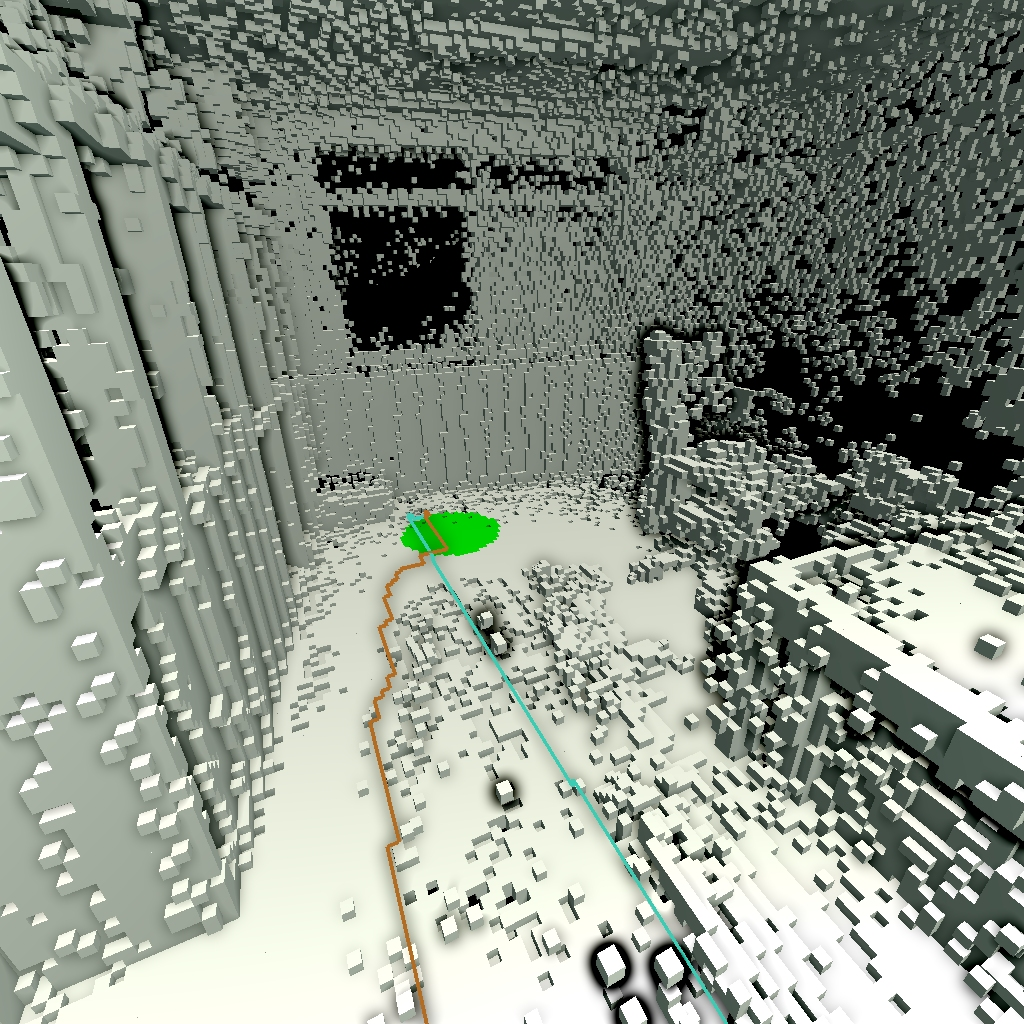
\includegraphics[height=0.255\linewidth]{figures/image1.jpg}}\label{fig:teaser:1}
	}
	\hfill
	\subfigure[Viable paths through offices with two hazardous environments highlighted.]{
		\fbox{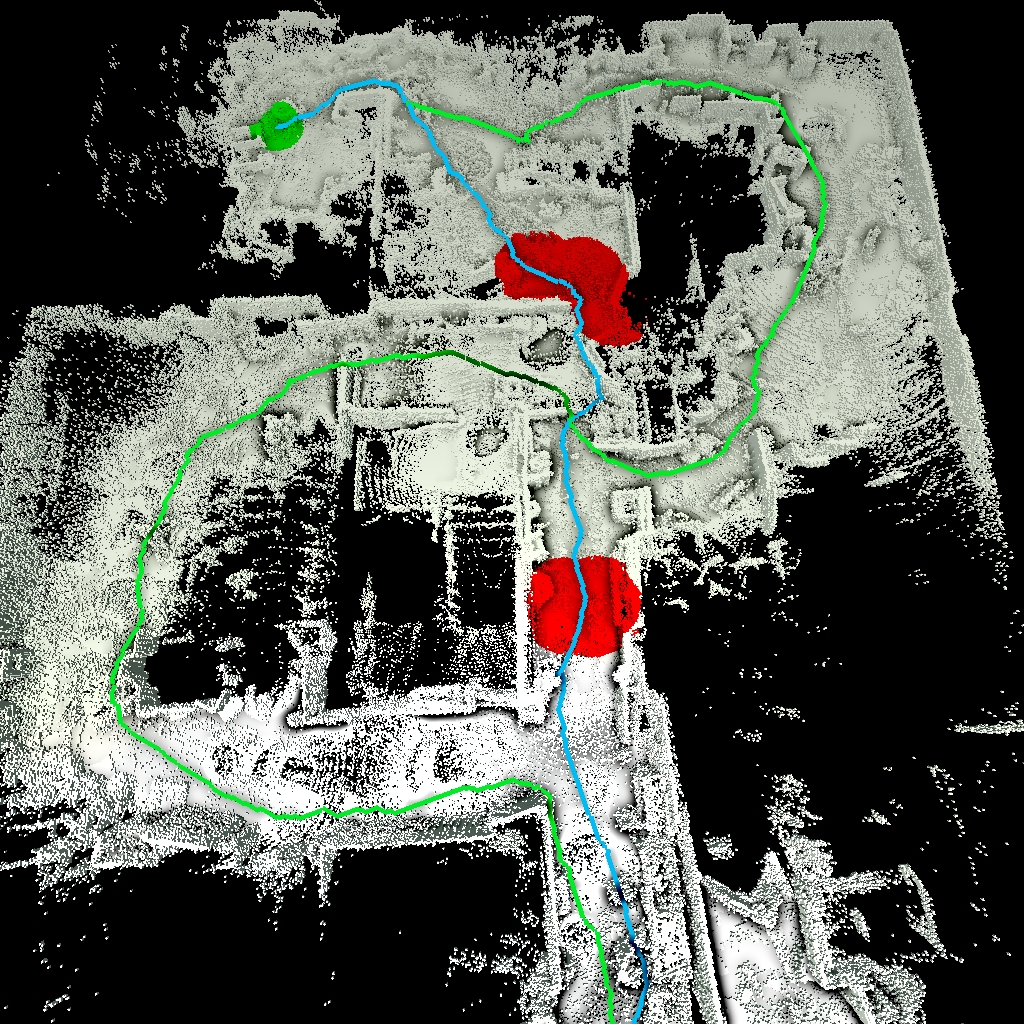
\includegraphics[height=0.255\linewidth]{figures/image2.jpg}}\label{fig:teaser:2}
	}
	\hfill
	\subfigure[Attributes derived in the data preprocessing stage. From left: distance to the closest hazard, occupancy, and level of support]{
	    \fbox{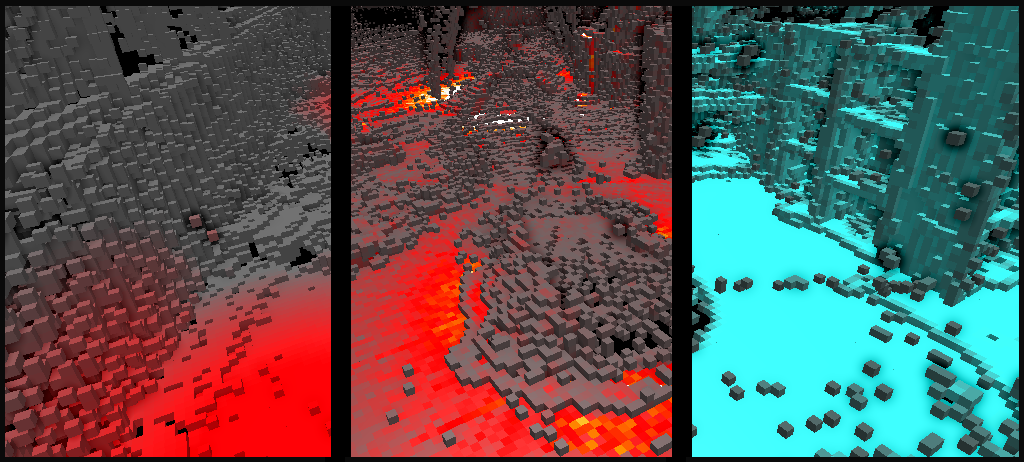
\includegraphics[height=0.255\linewidth, width=0.4\linewidth]{figures/fig-overview-fields-small.png}}
    \label{fig:overview:precomputation}
    }
%	\caption{(a) Attributes derived in the data preprocessing stage with values mapped to the colors of individual voxels, from left to right: distance to the closest hazard, occupancy or data density, and level of support.}	
%	\subfigure[Top-down view providing contextual information.]{
%		\fbox{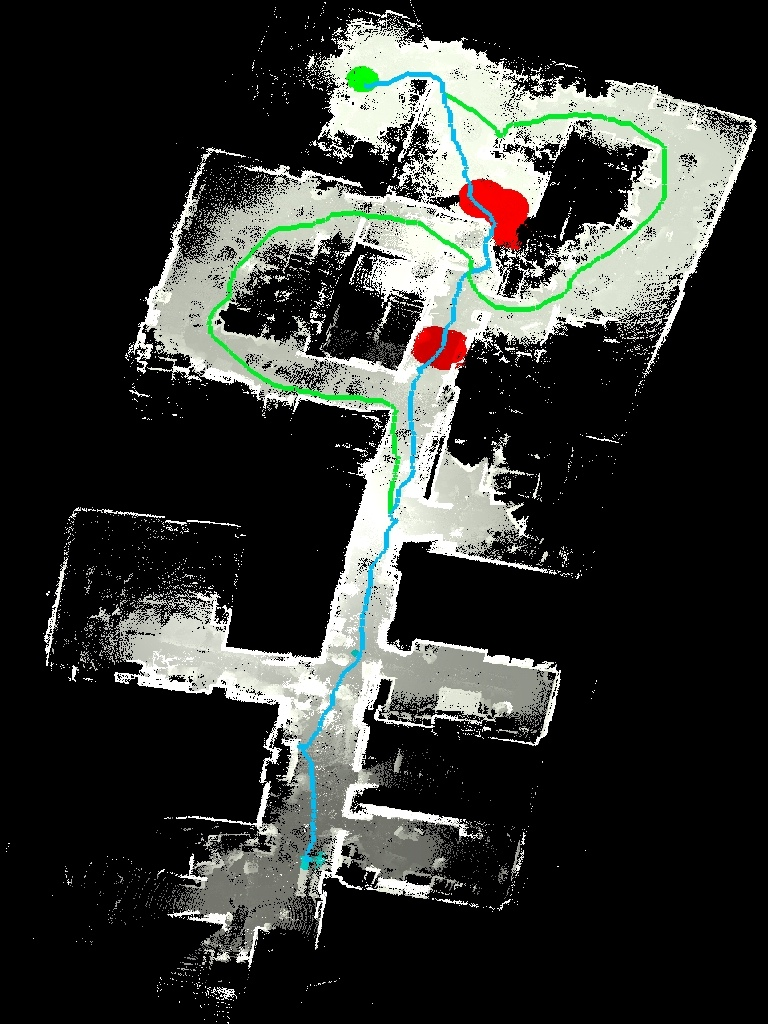
\includegraphics[height=0.25\linewidth]{figures/image2-overview.jpg}}\label{fig:teaser:3}
%	}
%	\hfill
%	\subfigure[In-depth analysis using parallel coordinates and profile plots.]{
%		\fbox{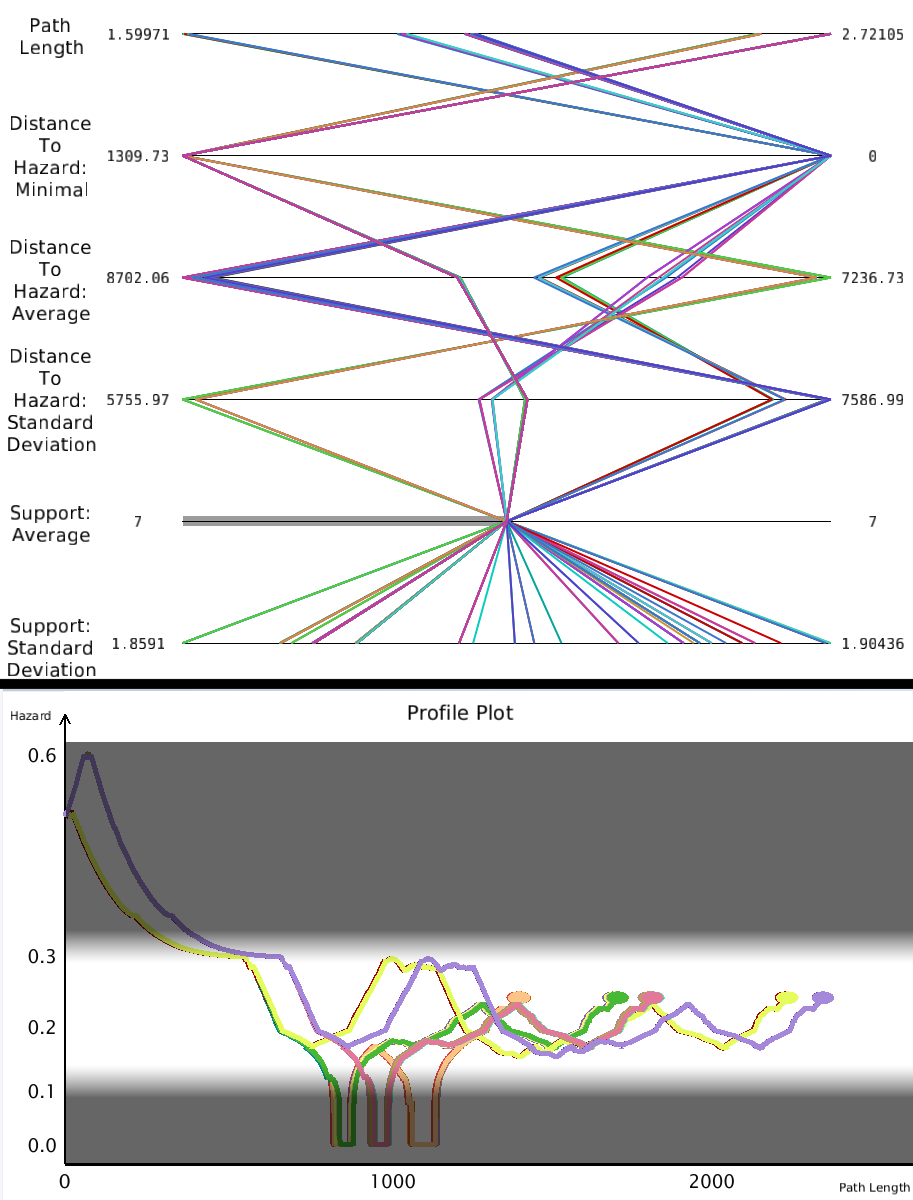
\includegraphics[height=0.25\linewidth]{figures/pcpprofile.png}}\label{fig:teaser:4}
%	}
  \caption{Our system applied to a building at Tohoku university. Different views support a comprehensive understanding, allowing the \IC\ to select and inspect paths that reach a point of interest, which are integrated into the rendering. Inspection and path computation is based on a set of derived attributes (c).}
  \label{fig:teaser}
\end{figure*}

Structural damage caused by disasters is an ever-present danger. As victims' survivability is mostly determined by the time-to-rescue, it is of great importance to provide medical attention or extraction as fast as possible. Planning access paths is, however, difficult as structural damage makes available floor plans outdated. In these situations, it is paramount that the \emph{Incident Commander} (IC) can analyze the available information and coordinate multiple rescue responders. There exist well-defined protocols to describe the phases in an \emph{Urban Search~\&~Rescue} (USAR) operation; in the assessment step, 2D maps of the collapsed buildings are hand-drawn based on the descriptions of rescue responders moving within the building searching for victims, possibly stumbling into hazardous areas that endanger the rescuer's life. In recent years, technological developments allowed unmanned vehicles to perform this initial exploration. The robots are equipped with sensors that can detect victims, gather information about hazardous environments, and perform scans of rooms to create a 3D point cloud of the building's interior. The \IC\ can inspect the building via the map and plan access paths that lead to \emph{Points of Interest} (POI), for example locations of victims, or other mission critical areas that need to be reached.

In this paper, we present a visualization system targeting search \& rescue situations. The system creates an interactive 3D rendering that increases the commander's spatial awareness of the building (Figures~\ref{fig:teaser}~(a-c) and~\ref{fig:cloud}) and supports the planning and analysis of access paths (Figure~\ref{fig:teaser}~(d)). The information is then used to instruct rescue responders to reach POIs and the \IC\ annotates the visualization with information provided by the on-site responders, thus shifting the decision making process from opportunistic to being strategical. Our system computes multiple access paths, each based on varying risk factors, and presents them to the \IC , allowing him to analyze and compare all available paths to minimize the rescuer's danger and travel time. We present design considerations with regard to decision making, technical realizations, and the results of an expert evaluation that show the usefulness and acceptance of this visualization system among professionals.

%%%%%%%%%%%%%%%%%%%%%%%%%%%%%%%%%%%%%%%%%%%%%%%%%%%%%%%%%%%%%%%%%%%%%%%%%%%%%%%%%%%%%%%%%%%
%%%%%%%%%%%%%%%%%%%%%%%%%%%%%%%%%%%%%%%%%%%%%%%%%%%%%%%%%%%%%%%%%%%%%%%%%%%%%%%%%%%%%%%%%%%

%\vspace*{-3pt}
\section{Related Work} \label{sec:relatedwork}
\noindent {\bfseries Emergency management.} Much of the visualization-oriented work published in the field of emergency management is concerned with pre-disaster evacuation planning. Notable work was performed by Reddy~\etal\ and is based on analyzing possible bottlenecks of escape routes~\cite{EuroVA12:13-17:2012}. While these algorithms could be utilized, they usually assume perfect walking conditions and a known layout of the building. Ribarsky~\etal\ presented a system organizing first responders in intact structures~\cite{Ribarsky:2010}. Kim~\etal\ developed a system enhancing the situational awareness of responders using a mobile visual analytics tool~\cite{Kim:2008}. Another related area is visual analysis-supported ensemble steering. Ribi\v{c}i\'c~\etal\ investigated steering ensembles of flooding simulations using visual analysis~\cite{6280550} and showed its usefulness to interpret this kind of data.

Many existing planning systems in USAR scenarios are based on 2D representations~\cite{kleiner_et_al_ssrr09,Pellenz2009SMU}. Given a 2D map, one approach to path planning is to use the shortest trajectory and follow it stepwise. Wirth~\etal\ introduced an exploration strategy and path planner that utilizes occupancy grid maps when planning to reach several targets simultaneously~\cite{Wirth2007ETA1}. Extensions towards exploration in 3D with regard to detection of voids were introduced by Dornhege and Kleiner~\cite{dornhege2011frontier}. In contrast to previous systems, our system's tight integration of 3D point cloud rendering, embedded access paths, and analysis tools enables a deeper immersion into the scene and thus improve the \IC 's decision-making process. 

\noindent {\bfseries Point cloud visualization.} Basic rendering capabilities for point clouds are offered by the widely used Point Cloud Library~\cite{Rusu11ICRA}. There has been work by Richter~\etal\ using a level-of-detail structure to render massive point clouds at high frame rates~\cite{Richter:2010:ORV:1811158.1811178}. Xu~\etal\ showed that non-photorealistic rendering techniques can be applied to point cloud data~\cite{conf/npar/XuC04}. The contour lines in their rendering inspired our rendering algorithm. More recently, Pintus~\etal\ presented a rendering algorithm that enhances features of unstructured point clouds in real-time without preprocessing~\cite{Pintus:2011:RRM:2384495.2384513}. In our system, we use a voxelized point cloud representation that raises the level of abstraction and simultaneously provides an immersive experience for the \IC . The binning of the point cloud data serves as a data reduction technique, increasing the performance of the rendering and thus immersion.

%%%%%%%%%%%%%%%%%%%%%%%%%%%%%%%%%%%%%%%%%%%%%%%%%%%%%%%%%%%%%%%%%%%%%%%%%%%%%%%%%%%%%%%%%%%
%%%%%%%%%%%%%%%%%%%%%%%%%%%%%%%%%%%%%%%%%%%%%%%%%%%%%%%%%%%%%%%%%%%%%%%%%%%%%%%%%%%%%%%%%%%

\section{Decision-Making Theory} \label{sec:theory}
In order to to design a system for USAR missions, it is crucial to utilize knowledge about human decision making. Decision makers in time-constrained situations tend to evaluate options serially; they attempt to find one viable plan rather than generating and comparing multiple plans in parallel. This theory has been described by Klein and Calderwood as \emph{Recognition Primed Decision-making} (RPD)~\cite{KleinCalderwood}. Initially, experts find similarities to previous cases, such as relevant goals, important things to monitor, and possible actions. Then, they simulate whether these parameters are also applicable to the current case.

The \emph{Contextual Control Model} (COCOM) by Hollnagel and Woods describes how people rely on context when making decisions~\cite{hollnagel2005joint}. The quality of their control can be described as scrambled, opportunistic, tactical, or strategic. The scrambled mode refers to decisions made without any information about the situation. In the opportunistic mode, people rely on cues in the local context to decide on their next action. In tactical mode, they have an idea of how to achieve their goal before taking action---a plan. In strategic mode, the plan includes coordination with other simultaneous goals. The goal of our system is to raise the quality of control from being opportunistic to being strategic, thus enabling improved decision-making.

The \emph{Extended Control Model} (ECOM) describes plans in terms of a tactical level (setting goals), monitoring (making plans and overseeing plans), regulating (managing local resources), and tracking (performing and adjusting actions)~\cite{hollnagel2005joint}. This theory is used to assess the kind of planning support a system provides. The importance of supporting resiliency has been argued by Lundberg~\etal : ``Rather than merely selecting a response from a ready-made table, [the system] must adapt and create a suitable response; either by following ready-made plans for adaptation or by making sense of the situation and create responses during the unfolding event''~\cite{Lundberg2012}.

%%%%%%%%%%%%%%%%%%%%%%%%%%%%%%%%%%%%%%%%%%%%%%%%%%%%%%%%%%%%%%%%%%%%%%%%%%%%%%%%%%%%%%%%%%%
%%%%%%%%%%%%%%%%%%%%%%%%%%%%%%%%%%%%%%%%%%%%%%%%%%%%%%%%%%%%%%%%%%%%%%%%%%%%%%%%%%%%%%%%%%%

\section{Incident Commander Workflow} \label{sec:workflow}
%
%%\begin{figure}
%%	\centering
%%	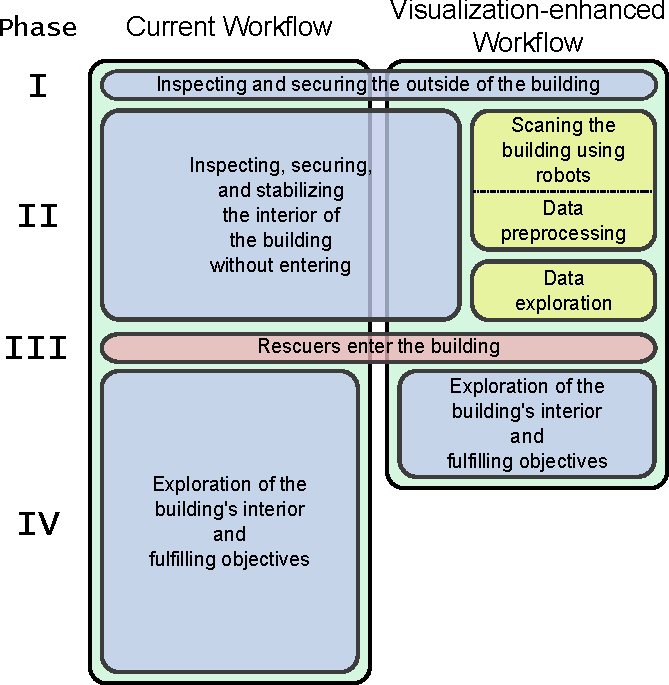
\includegraphics[width=0.9\columnwidth]{figures/workflow.pdf}
%%	\caption{A schematic timeline overview of the currently employed workflow (left) and our proposed visualization-enhanced system (right), showing all events (red) and actions (blue) split up into five distinct phases (roman numerals). Utilizing the additional actions (yellow) in parallel and thus enabling faster and less dangerous exploration, we decrease the overall time-to-rescue.}
%%	\label{fig:workflow:workflow}
%%\end{figure}
%
In most USAR protocols, one \IC\ is responsible for a single building and instructs multiple rescue responders inside this building. In this section, we will describe our visualization-enhanced workflow supporting the \IC\ in this task.

%
%\noindent {\bfseries Current workflow.} After arriving at the disaster scene (Phase \texttt{I}), the first step for the responders is to explore and secure the area outside the collapsed building (Phase \texttt{II}). No rescuer is allowed to enter the building before it is secured, which can take an hour or more to finish (Phase \texttt{III}). Then, based on the gathered information, the \IC\ determines valid entry points into the structure and directs rescuers into the collapsed structure to perform reconnaissance (Phase \texttt{IV}). Using constant radio communication, the rescuer inside the building slowly advances and reports his progress to the \IC, who draws a 2D map (see Figure~\ref{fig:workflow:sota}) based on that information (Phase \texttt{V}). The rescuer enters the unknown building with unquantifiable risks, like gas leaks or dormant fires, inside. Not only is the 2D drawing of an unstructured 3D building insufficient and inaccurate, it also does not provide acceptable spatial awareness. This is clearly an example of opportunistic control, where decisions are made opportunistically based on feedback from the environment. The map is created as the rescuer proceeds, inhibiting higher levels of control in the beginning of the path. Although responders may recognize situations, decisions regarding the path are limited to the extent of the current exploration and to their view of the local environment. Initially, therefore, any RPD is restricted to the local environment. Global planning is limited further by the ability of responders to communicate relevant structural information accurately to the \IC, such as angles of turns, which cause hand-drawn maps to experience drift. This technique of opportunistic exploration has further limitations in that a faster and safer path might exist, but is not known to the rescuer or the \IC\ at that moment.
%
After arriving on location, the responders' first step is to explore and secure the outside of the collapsed building. No rescuer is allowed to enter the building before it is secured, which can take an hour or more to complete. During this step, unmanned vehicles record and measure the inside of the building, feeding back information to the \IC , who inspects the map and determines entry points combining the map information with real-world input. The robots' sensors are able to detect most signs of victims using various sensors~\cite{Wu12Eulerian}, but as these measurements are uncertain, both false positives and false negatives might occur. The same holds true for hazardous environments like fires, gas leaks, radiation, or structurally unsafe areas. The data retrieval and preprocessing is done in parallel with securing the perimeter so that all information is available when the next phase begins. Based on suggested or selected POIs, the system computes optimal paths that the \IC\ uses to direct the rescuers through the building. This reduces time-to-rescue as the rescuers do not need to explore the building to the same extent, but can proceed directly to the POIs. Thus, the system applies RPD to the whole situation, extending the number of available cues and planning from local conditions to higher ECOM levels.

When planning access paths, a variety of factors must be taken into account. The responder has to, among others, maintain a safe distance from hazardous environments, avoid overhanging structures, and the ground must be level. Uncertainty in the data and \IC 's invaluable knowledge make an algorithm for the problem infeasible. Furthermore, as these variables are extracted from uncertain data, they are difficult to quantify and subject to uncertainties. The \IC\ has to perform trade-offs to choose between alternatives, for example favoring a faster, longer path over a more dangerous, shorter path.

While the \IC\ instructs a rescuer to follow one path, new information about victims or hazards is fed back which the \IC\ incorporates into the system. This feed-back loop is of high importance as features might not only have been missed by the robots, but detected features might change during the rescue operation. Fires can start or extinguish, structural collapses can make areas inaccessible, or debris is removed after the initial reconnaissance, opening previously inaccessible areas. 

%%%%%%%%%%%%%%%%%%%%%%%%%%%%%%%%%%%%%%%%%%%%%%%%%%%%%%%%%%%%%%%%%%%%%%%%%%%%%%%%%%%%%%%%%%%
%%%%%%%%%%%%%%%%%%%%%%%%%%%%%%%%%%%%%%%%%%%%%%%%%%%%%%%%%%%%%%%%%%%%%%%%%%%%%%%%%%%%%%%%%%%

\section{System Overview} \label{sec:overview}
%Combining expertise in visualization, cognitive systems engineering, rescue robotics, and thorough discussions with domain experts, we determined a set of requirements that must be fulfilled to make our system useful for the \IC. We employed theories from sense-making and decision-making (see Section~\ref{sec:theory}) to guide the design of our system to fully support the \IC. The visualization components are designed to comply with these theories and have been tested in a user study with external domain experts as described in Section~\ref{sec:evaluation}.
%
%The components should fulfill the following requirements, which we have derived from our discussions with the collaborating experts:
%
%\begin{description}
%\item[R1] The system must increase the \IC 's spatial awareness by allowing for interactive exploration of the collapsed structure.
%\item[R2] The system must enable the \IC\ to interactively annotate the acquired data to react to changing circumstances in the structure.
%\item[R3] The \IC\ must be able to inspect multiple access paths and be able to compare them and make trade-offs.
%\item[R4] The system must provide the tools to select a globally optimal path and allow for its execution.
%\end{description}

%The proposed system employs multiple linked views to address these requirements (see Figure~\ref{sec:overview:system}). In order to fulfill requirement {\bfseries R1}, our system visualizes the acquired point cloud in an interactive manner that preserves occlusion and helps the \IC\ to form a consistent mental model of the structure. Within this visualization, the \IC\ can seamlessly annotate newly discovered entrances, hazards, POIs, and forbidden areas, thus fulfilling requirement {\bfseries R2}. To address requirements {\bfseries R3} and {\bfseries R4}, we integrate a visual representation of the different paths into the 3D visualization, and provide separate in-depth analysis tools.

Our proposed system employs multiple linked views to provide the \IC\ with all information (see Figure~\ref{sec:overview:system}). The following sections explain these components. Before the acquired data can be used, a preprocessing must be performed that extracts derived data from the point cloud data (Section~\ref{sec:overview:preprocessing}). Then, interactive data annotation is possible (Section~\ref{sec:overview:annotation}). The generation of the optimal access paths, together with the employed metric, is explained in Section~\ref{sec:overview:pathcomputation}. Section~\ref{sec:overview:3dvisualization} provides details on the design considerations for the 3D visualization component of our system and the analysis of the path ensemble is described in the Section~\ref{sec:overview:pathanalysis}.

\begin{figure}
    \centering
    \fbox{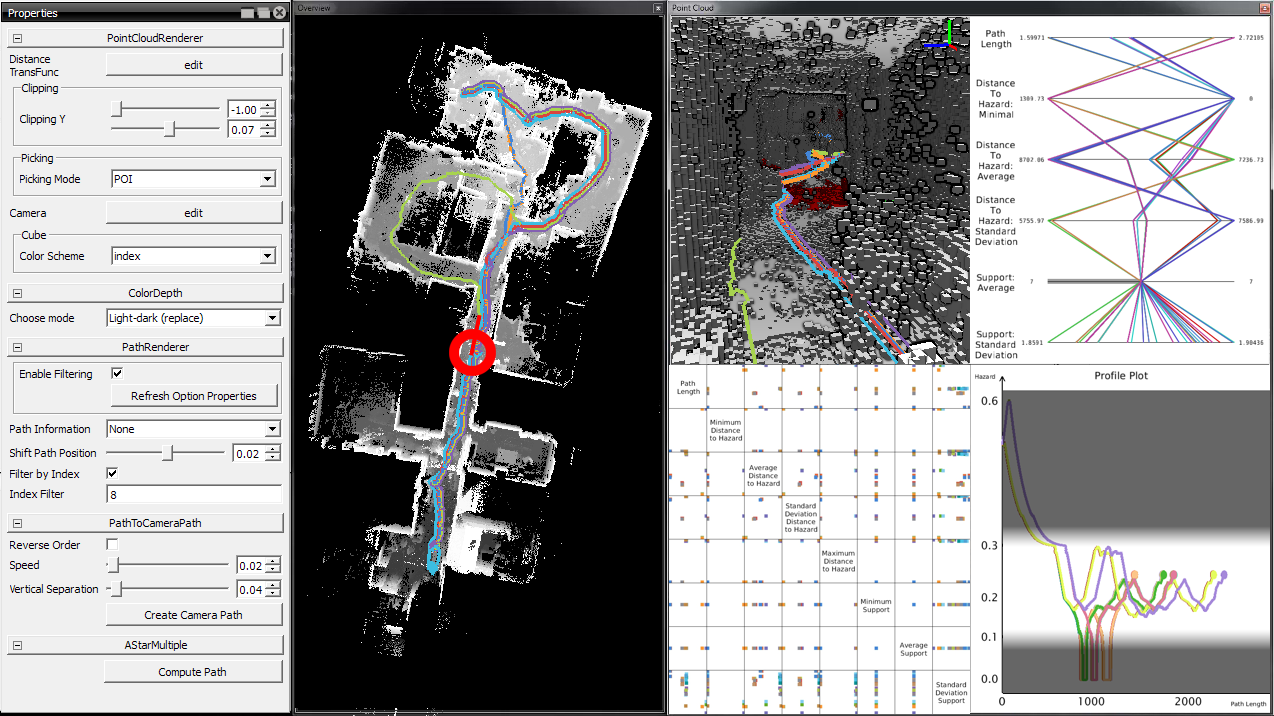
\includegraphics[width=\columnwidth]{figures/fig-overview-system2.png}}
    \caption{A screenshot showing our system for a typical scenario. Each view can be maximized to fill the entire screen for in-depth inspection. An overview (left) shows a top-down view of the building to provide context, a multi-view (right) shows the different components of our system.}
    \label{sec:overview:system}
\end{figure}

\subsection{Data Preprocessing} \label{sec:overview:preprocessing}
The data retrieved from the unmanned robots is an unstructured 3D point cloud. One issue with directly rendering such point clouds is missing occlusion information and the non-uniform distribution of points. To avoid this problem, we perform a binning of the point cloud to obtain a three-dimensional voxel structure on a regular grid. From this point, we call a measurement in the original point cloud a \emph{point} and refer to a position in the grid-based, binned point cloud as a \emph{voxel}. After the binning, the resulting regular structure contains one voxel for all bins with at least one point. The bin size is dependent on the scan resolution of the robot, as it is a trade-off between resolving smaller details and decreasing SNR. In our cases, sizes of about 5\,cm were sufficient. Figures~\ref{fig:cloud}(f--h) show three examples of possible voxel sizes obtained from the Jacobs University's Rescue arena dataset.

In the second part of the preprocessing, derived attributes are computed that are later used to determine the set of access paths and to support their analysis. We compute the \emph{hazard distance field} (Figure~\ref{fig:overview:precomputation} left) that denotes the distance to the closest hazard points for each voxel, weighted by severity. The \emph{occupancy field} (Figure~\ref{fig:overview:precomputation} center) denotes the number of points each voxel is based on. A higher occupancy means that the voxel covers more points in the original point cloud and thus provides a higher certainty. The \emph{support field} (Figure~\ref{fig:overview:precomputation} right) shows the available supporting area for each voxel. This value determines whether there is enough floor available for a responder to walk without hindrance. The \emph{size field} shows for each voxel if a rescuer can fit into the space above without squeezing. We calculate two size values, one with the rescuer standing up, and a second while crouching. We also require orientation information to be able to exclude paths that would be too steep for a rescuer. For this, we compute the least-squares fitted plane based on all the points that are covered by a voxel. The normal of the plane is then used for the voxel.

\begin{figure*}
    \newlength{\mywidth}
    \setlength{\mywidth}{0.23\textwidth}
    \centering
    \subfigure[Unstructured, unbinned rendering of individual points hindering immersion]{
        \fbox{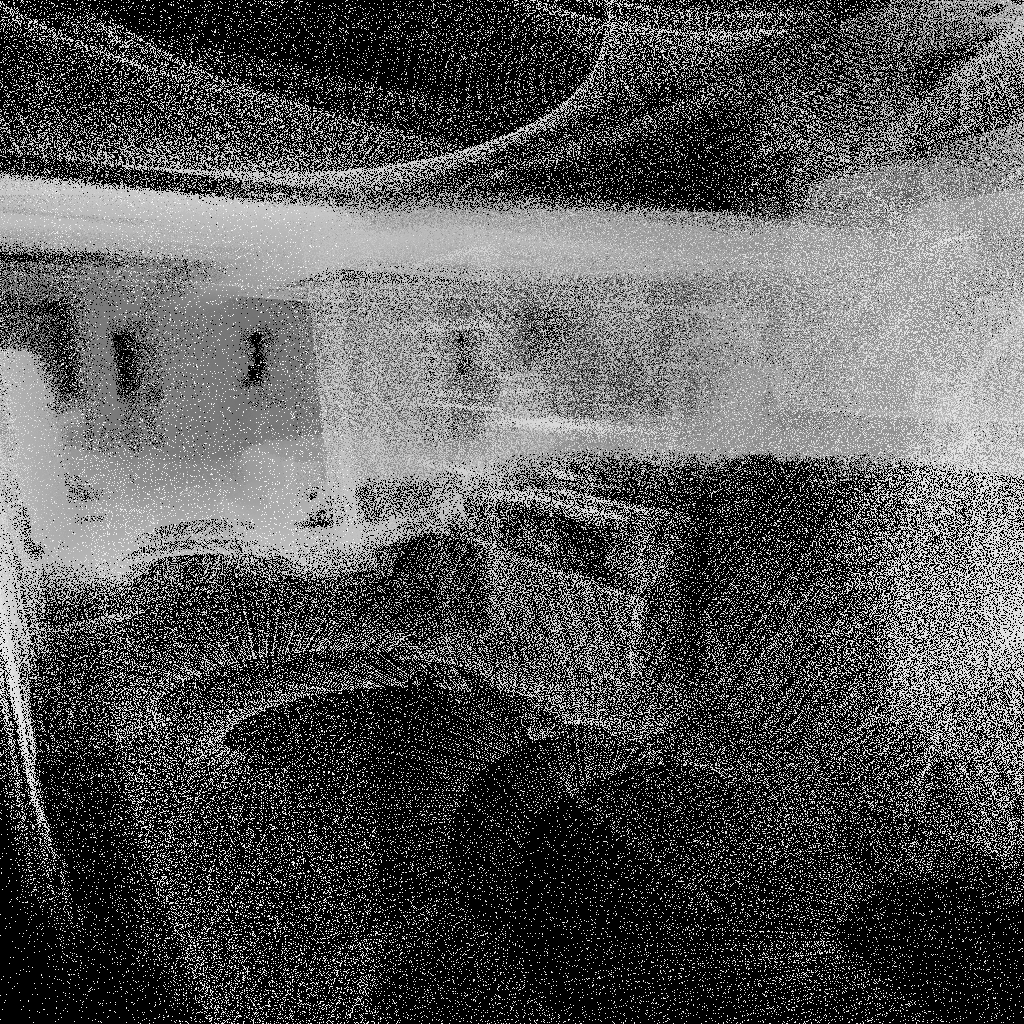
\includegraphics[width=\mywidth]{figures/fig-rendering-points.png}}
        \label{fig:cloud:points}
    }
    \hfill
    \subfigure[Unenhanced voxelized rendering containing only lighting information]{
        \fbox{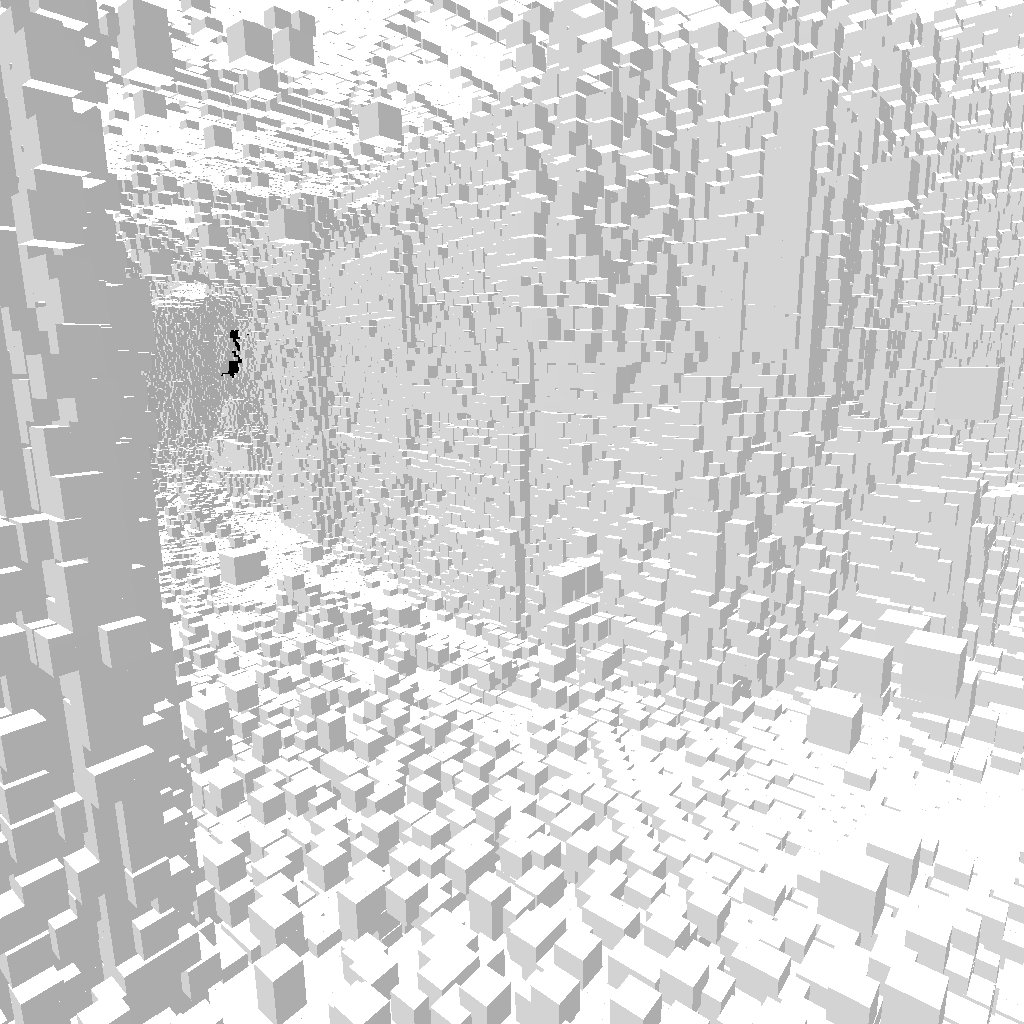
\includegraphics[width=\mywidth]{figures/fig-rendering-default.png}}
        \label{fig:cloud:default}
    }
    \hfill
    \subfigure[Full voxelized rendering with contour and depth enhancements]{
        \fbox{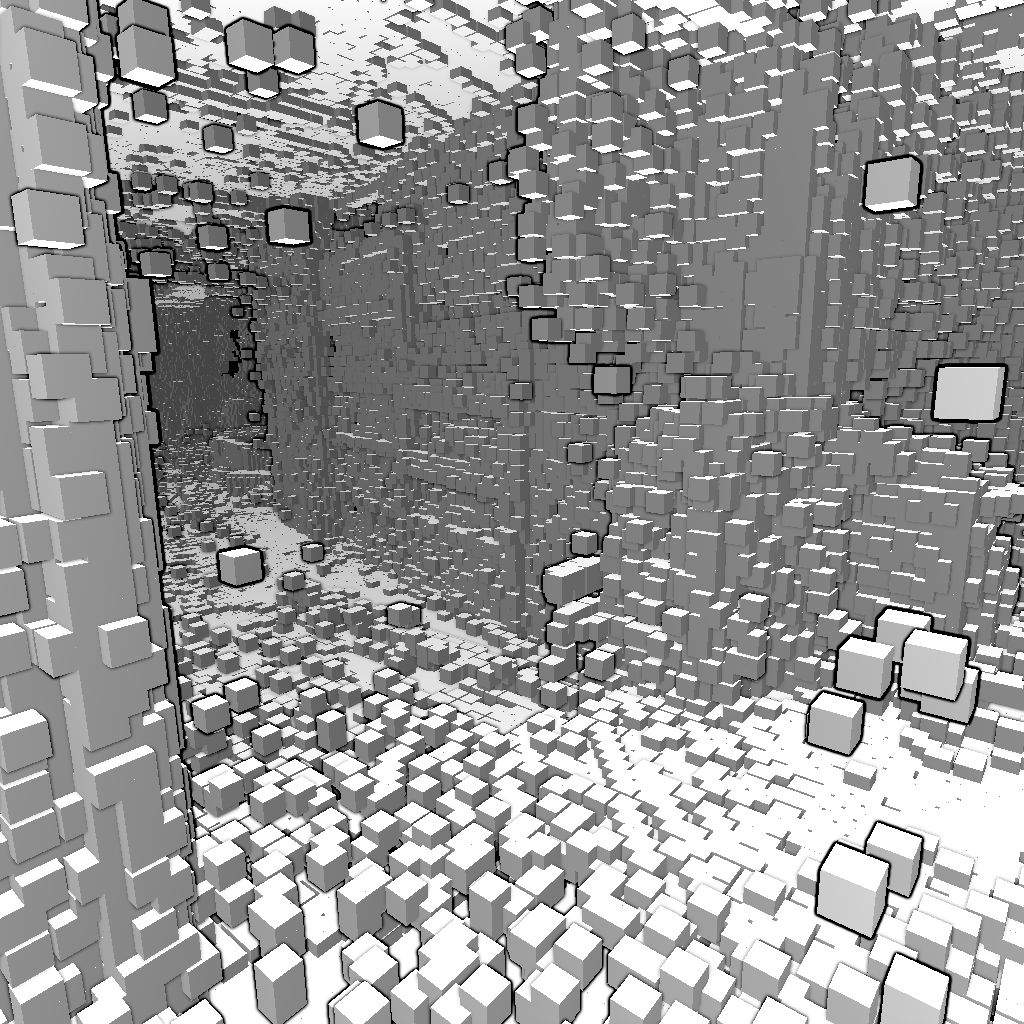
\includegraphics[width=\mywidth]{figures/fig-rendering-voxel.png}}
        \label{fig:cloud:voxel}
    }
    \hfill
    \subfigure[Depth-image rendering emphasizing the overall structure of the corridor]{
        \fbox{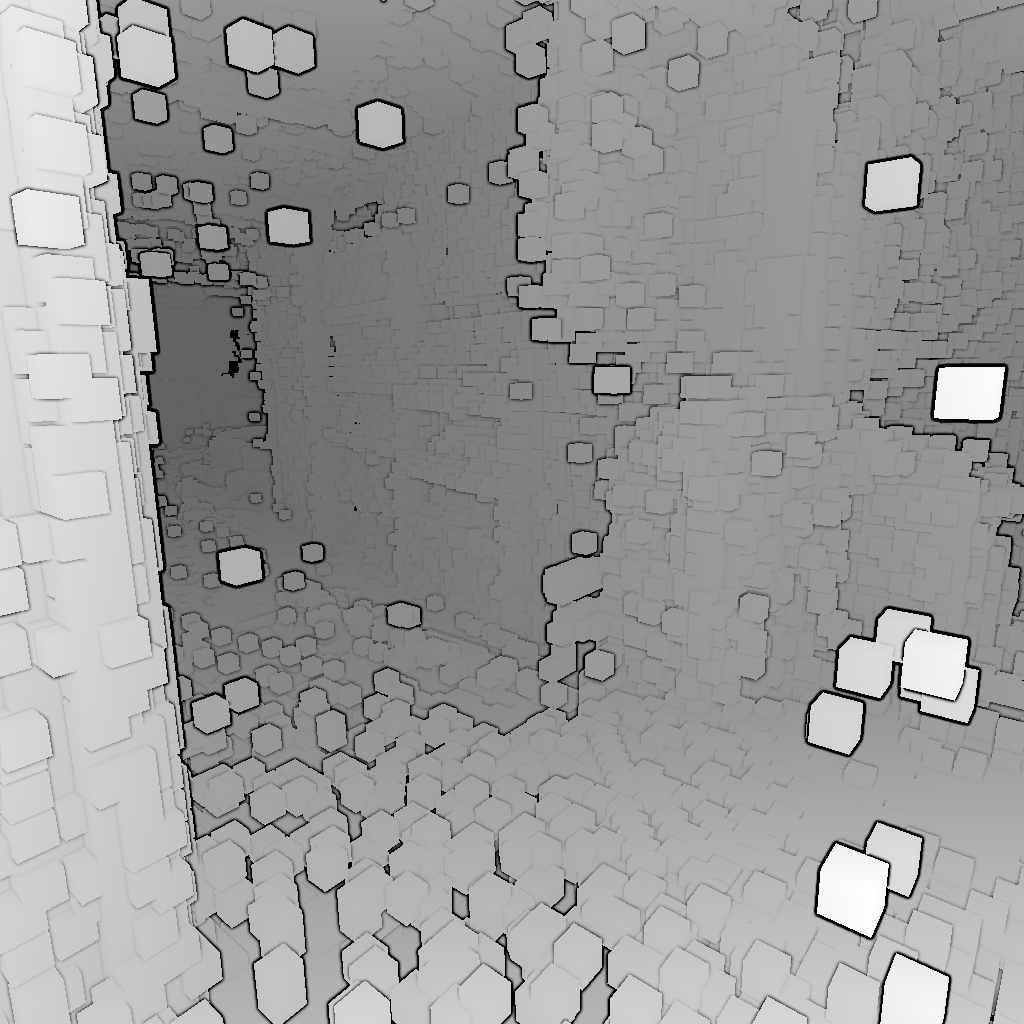
\includegraphics[width=\mywidth]{figures/fig-rendering-depth.png}}
        \label{fig:cloud:depth}
    }
    \\
    \subfigure[Stereoscopic fisheye rendering used for full-dome projection systems]{
        \fbox{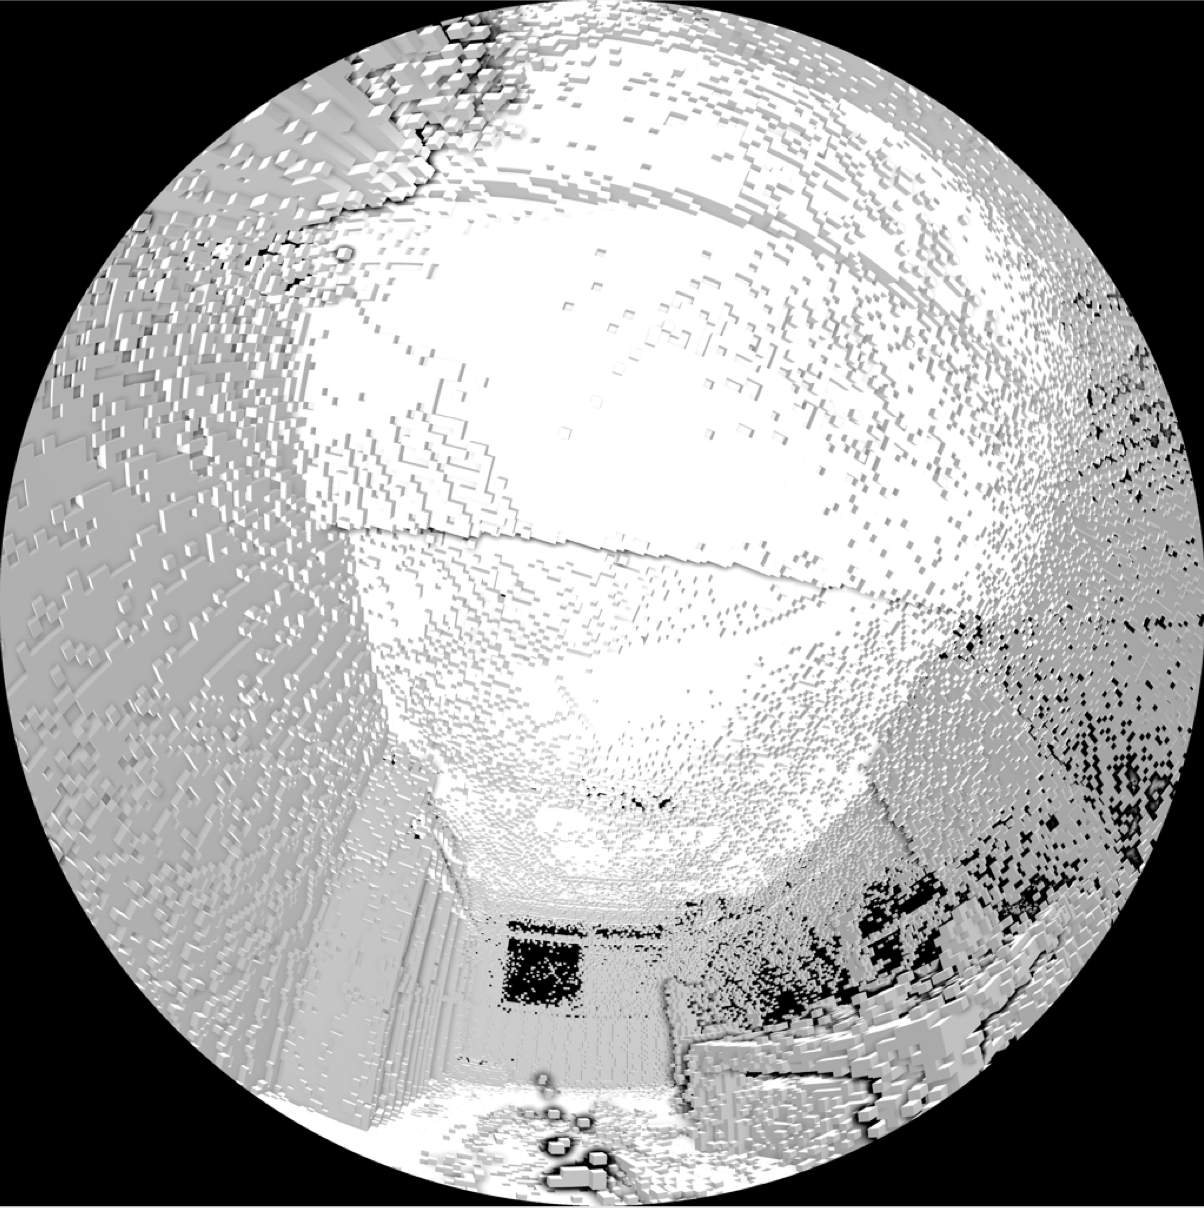
\includegraphics[width=\mywidth]{figures/fig-dome.png}}
        \label{fig:cloud:dome}
    }
    \hfill
    \subfigure[The Jacobs University rescue arena data set with $4 \times 4 \times 4$ cm voxels]{
        \fbox{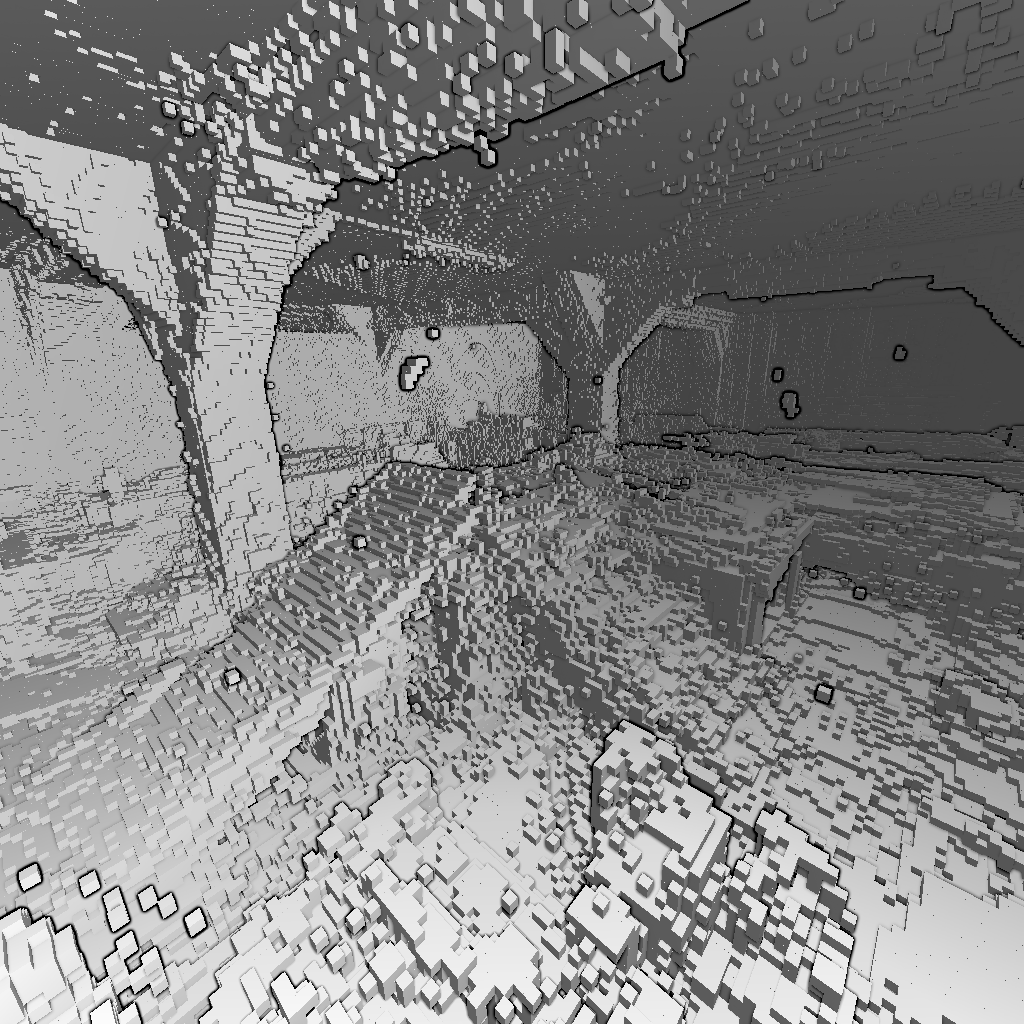
\includegraphics[width=\mywidth]{figures/fig-rescue-4.png}}
        \label{fig:cloud:4}
    }
    \hfill
    \subfigure[The Jacobs University rescue arena data set with $10 \times 10 \times 10$ cm voxels]{
        \fbox{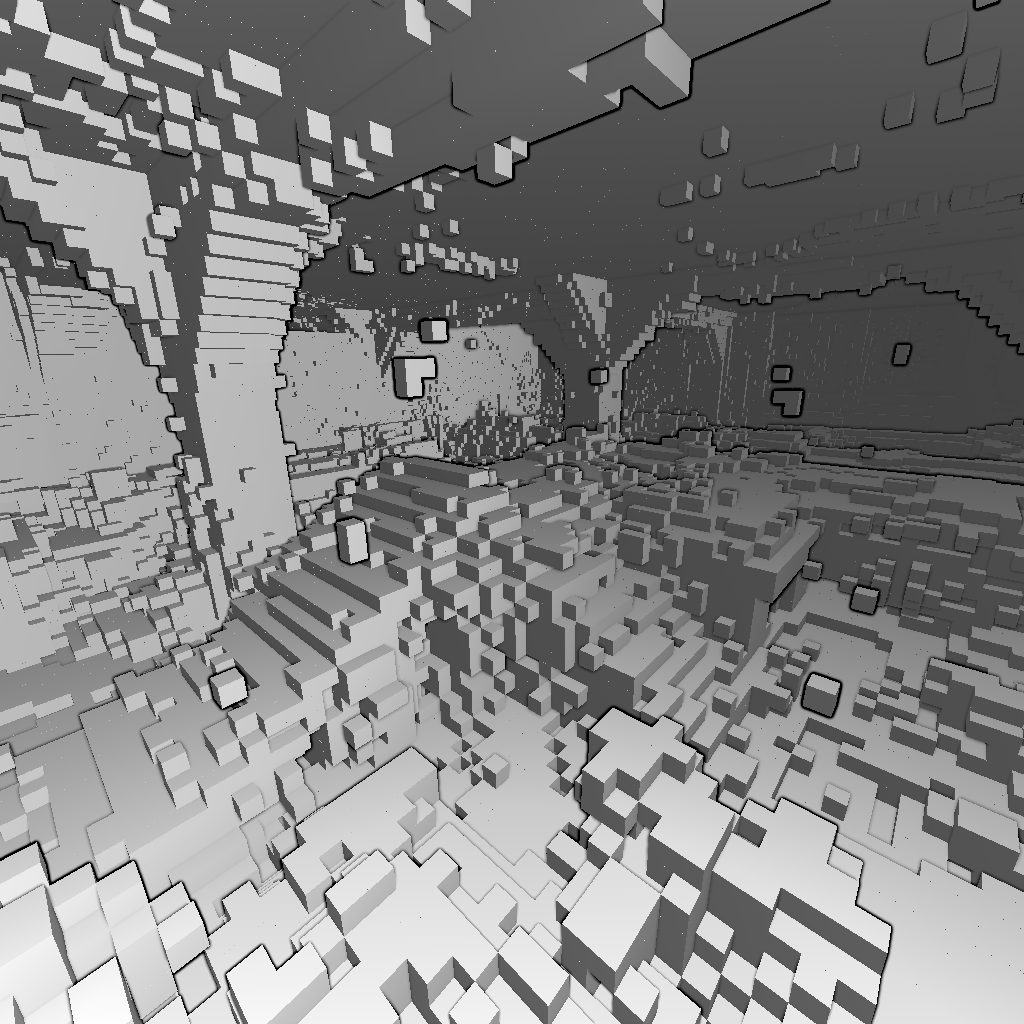
\includegraphics[width=\mywidth]{figures/fig-rescue-10.png}}
        \label{fig:cloud:10}
    }
    \hfill
    \subfigure[The Jacobs University rescue arena data set with $25 \times 25 \times 25$ cm voxels]{
        \fbox{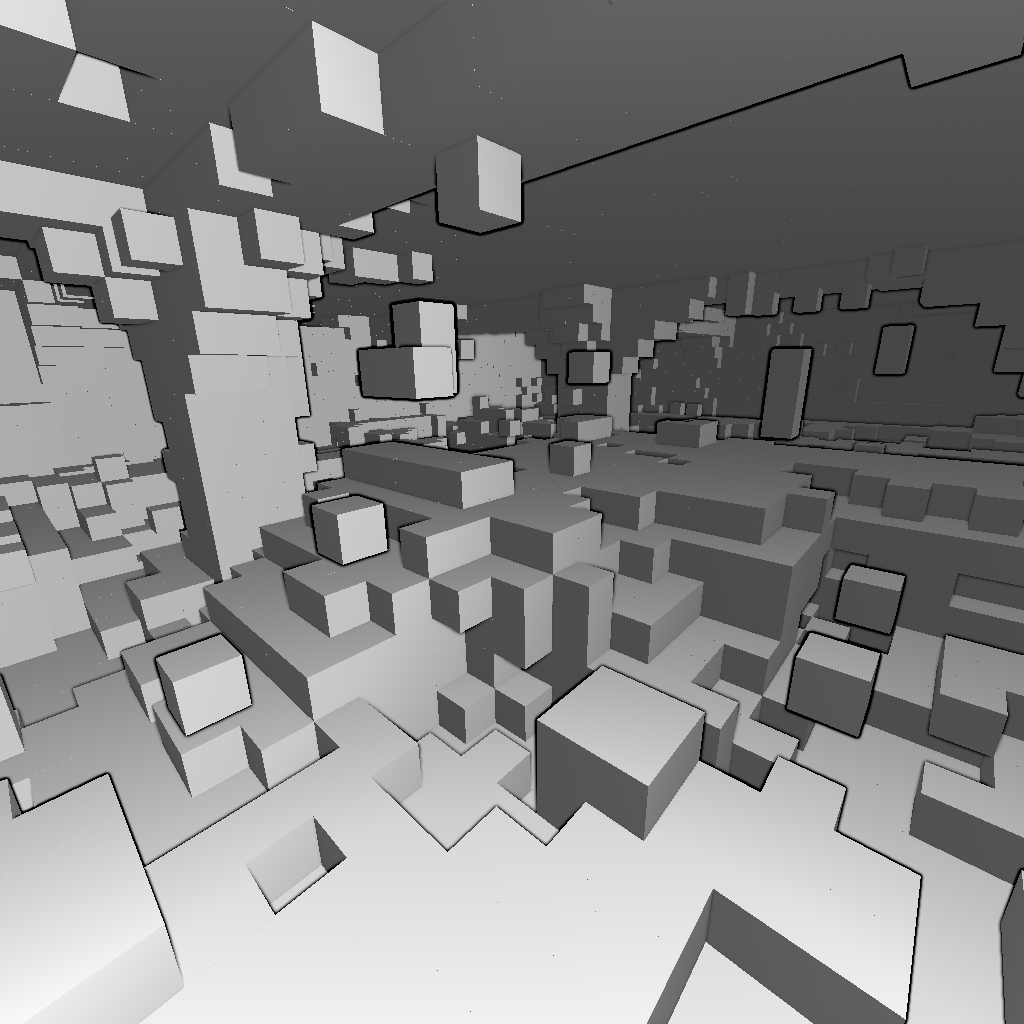
\includegraphics[width=\mywidth]{figures/fig-rescue-25.png}}
        \label{fig:cloud:25}
    }
    \caption{These images show different rendering techniques of the same location in the Tohoku dataset (a--d). Rendering the individual voxels as points does not allow for an immersive rendering as depth-cues are missing (a). Binning the point cloud and representing each voxel as a axis-aligned box solves this problem (b). In order to enhance the contours of the scene and produce a better immersion, we perform image-space enhancements (c). Alternatively, the \IC\ can choose a rendering method imitating the output of range imaging cameras (d). It is possible to render the point cloud in stereoscopic fisheye that can be used for dome surfaces or VR glasses (e). The voxel size's effect during binning is shown for the rescue arena dataset (f--h).}
    \label{fig:cloud}
\end{figure*}


%\begin{figure}
%    \centering
%	\subfigure[Unstructured point cloud]{
%    	\fbox{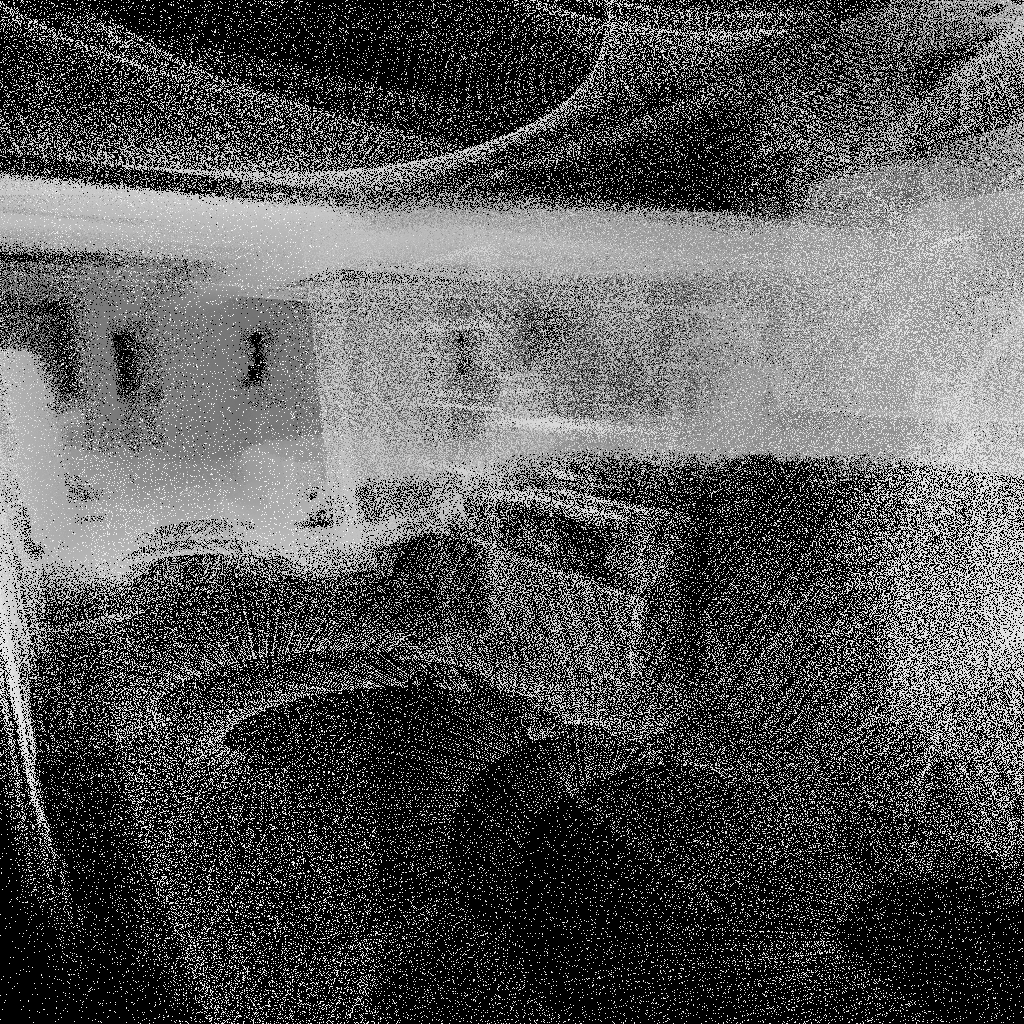
\includegraphics[width=0.29\columnwidth]{figures/fig-rendering-points.png}}
%    	\label{fig:cloud:points}
%	}
%	\hfill
%	\subfigure[Voxelized point cloud]{
%	    \fbox{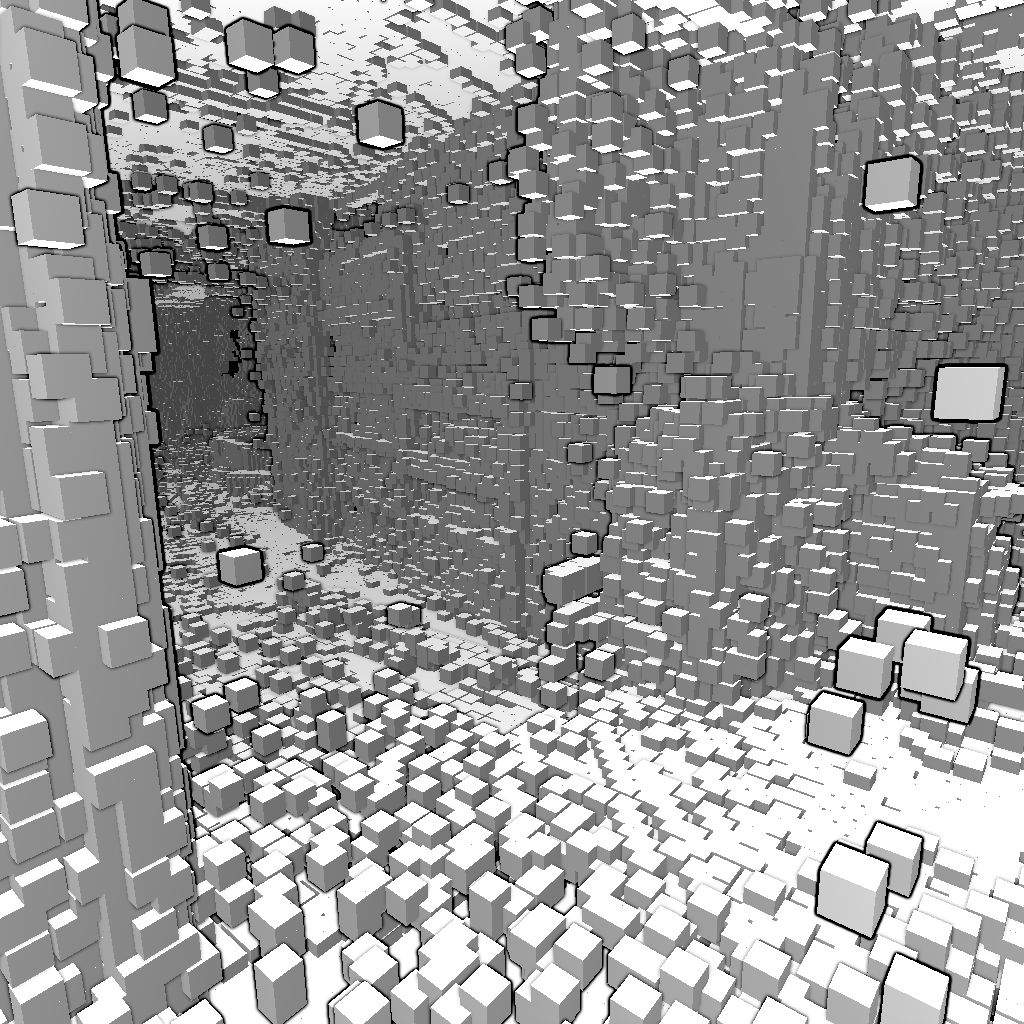
\includegraphics[width=0.29\columnwidth]{figures/fig-rendering-voxel.png}}
%	    \label{fig:cloud:voxel}
%	}
%	\hfill
%	\subfigure[Depth-image]{
%	    \fbox{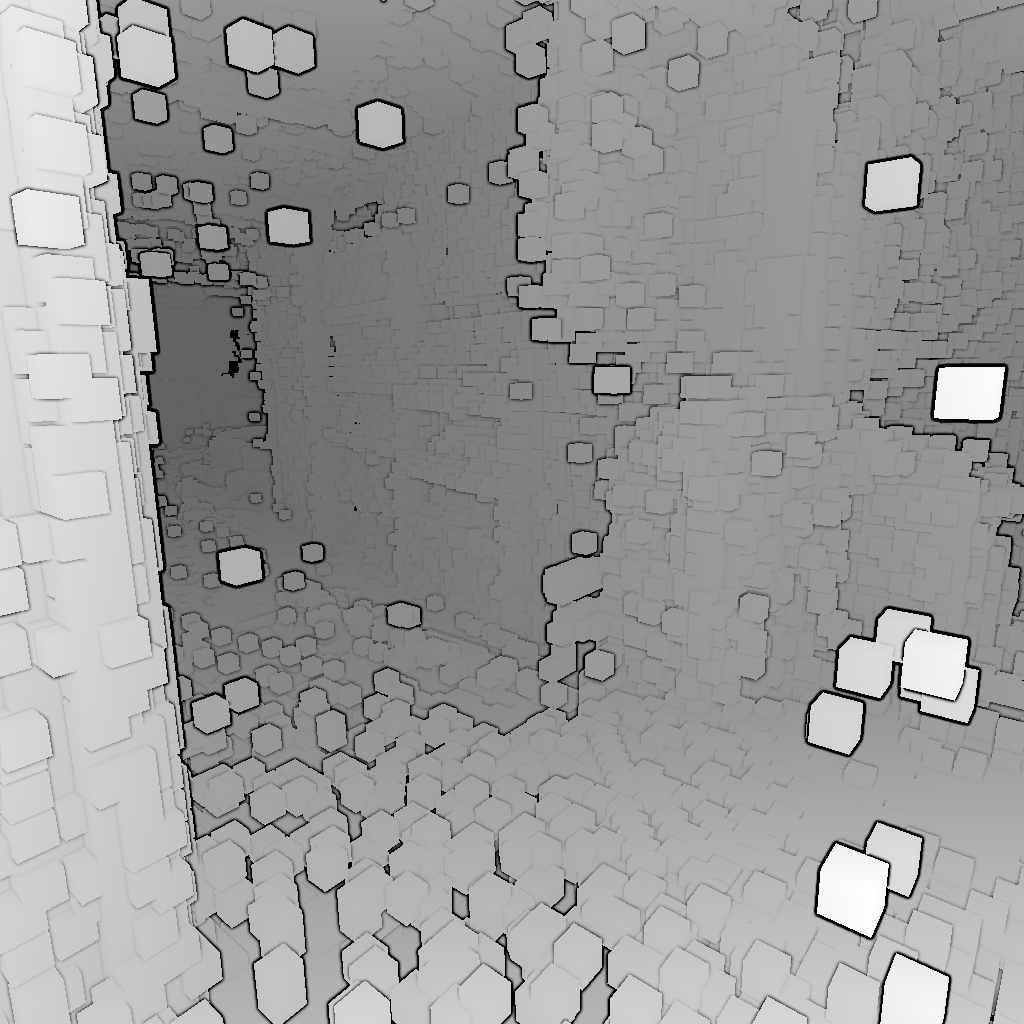
\includegraphics[width=0.29\columnwidth]{figures/fig-rendering-depth.png}}
%	    \label{fig:cloud:depth}
%	}
%	\caption{Screenshots using two different rendering techniques for the point cloud data for the identical scene and camera position. (a) shows the unstructured point cloud where each point is rendered at its correct position, but no depth cues are present in the rendering thus not facilitate easy spatial recognition. (b) shows the point cloud after the resampling has been performed and each point is rendered as an axis-aligned, opaque, and shaded box. This enhances the depth perception and allows the structure of the data to be seen.}
%\end{figure}
%
%\begin{figure}
%   \centering
%   \subfigure[$4 \times 4 \times 4$ cm]{
%       \fbox{\includegraphics[width=0.29\columnwidth]{figures/fig-voxelsize-4.jpg}}
%   }
%   \hfill
%   \subfigure[$10 \times 10 \times 10$ cm]{
%       \fbox{\includegraphics[width=0.29\columnwidth]{figures/fig-voxelsize-10.jpg}}
%   }
%   \hfill
%   \subfigure[$25 \times 25 \times 25$ cm]{
%       \fbox{\includegraphics[width=0.29\columnwidth]{figures/fig-voxelsize-25.jpg}}
%    }
%   \caption{The influence of the voxel size on a dataset scanned at the rescue arena at the Jabobs University in Bremen. The voxel size is a trade-off between higher detail and higher data uncertainty.}
%   \label{fig:overview:precomputation:voxelsize}
%\end{figure}
%
\subsection{Data Annotation} \label{sec:overview:annotation}
It is essential to be able to classify and annotate the data interactively. In our system, each voxel can belong to one of five classes. \emph{Unclassified} is the default class and does not convey any semantics. \emph{Start} voxels are usable entry points from which paths can start. \emph{POI} voxels are destination points for a path and indicate a potential victim or another mission-critical element. \emph{Hazard} voxels have been declared as dangerous due to, for example, an ongoing fire or gas leak. \emph{Forbidden} voxels can only be declared by the \IC\ and are areas completely out of reach for traversal. The \IC\ modifies the classification for each voxel by interacting directly with the point cloud rendering.

\subsection{Path Computation} \label{sec:overview:pathcomputation}
We employ the widely used A* algorithm for our path computations~\cite{4082128}. It is a best-first search algorithm that works as follows: For the current point $\mathbf{p}$, the estimated remaining distance is calculated for each unvisited neighboring point $\mathbf{q}$. This value is the sum of the cost to reach $\mathbf{p}$ from the start, the cost to move from $\mathbf{p}$ to $\mathbf{q}$, and the estimated cost to reach the target from $\mathbf{q}$. Then, the point with the lowest cost is chosen as the next valid point to be tested. For a comprehensive description of the algorithm we refer the reader to the book by Russel and Norvig~\cite{AStar}. When computing a path with A*, a metric is used that determines the cost of moving from one point to its neighbor. Thus, it is possible to compute several optimal paths by changing this metric. Our metric is composed of weighted sub-metrics that are summed to yield

\begin{equation}
\begin{array}{r@{}l}
m = & \textrm{L}_2(\mathbf{p},\mathbf{q}) + w_h \cdot \textrm{hazard}(\mathbf{q}) + w_s \cdot \textrm{size}(\mathbf{q}) + \vspace*{0.1cm} \\
  & w_n \cdot \textrm{normal}(\mathbf{q},\varphi) + w_{sup} \cdot \textrm{support}(\mathbf{q},n)
\end{array}
\end{equation}

\noindent where $w_h$, $w_s$, $w_n$, and $w_{sup}$ are the weights that are varied between different runs of the path computation. $\textrm{hazard}(\mathbf{q})$ returns the hazard severity that is stored in the hazard field. $\textrm{size}(\mathbf{q})$ is a binary function that determines if there is enough space above the voxel $\mathbf{q}$. The $\textrm{normal}(\mathbf{q},\varphi)$ function computes the surface normal for $\mathbf{q}$ and returns a normalized, linear response between the maximum allowed deviation $\varphi$ and the gravity vector. $\mathrm{support}(\mathbf{q},n)$ is dependent on the number of supporting voxels in the area around the point $\mathbf{q}$ and is retrieved from the support field. Here, $n$ is a threshold determining how many voxels are needed to consider $\mathbf{q}$ being supported.

\subsection{3D Visualization} \label{sec:overview:3dvisualization}
\noindent {\bfseries Point cloud visualization.} Missing occlusion, and thus missing depth cues, is a big challenge in point cloud rendering. Rendering each point individually inhibits immersion as structural features are hard to detect (Figure~\ref{fig:cloud:points}). One attempt to add occlusion is to apply stencilling by rendering orthogonal disks around each point. Using this approach, points will have camera-aligned occlusion zones in which no points are rendered. This fails for several reasons; the size of the occlusion zone depends on the sparseness of points and if the zone is chosen too small otherwise occluded points will be visible. Second, the occlusion zone will also hide points belonging to the same structure. This leads to the structure, for example a wall, being represented only by a few points which does not reflect reality. Utilizing a voxelized representation was beneficial in which each voxel is represented by an axis-aligned cube with the same size as the grid structure. Figure~\ref{fig:cloud:default} shows the result of this rendering method. This technique solves the occlusion problem immediately, as each voxel has an extent and occludes voxels. Only in cases with very sparse data do holes appear in the rendering. To increase the spatial awareness, we apply a lighting based on the face of the cube, rather than the normal of the voxel. We decided to utilize two image-space enhancement techniques to increase the immersion. The first method, presented by Luft \etal~\cite{Luft06imageenhancement}, is a contour-enhancement that increases local contrast in areas of high depth changes. This allows the \IC\ to intuitively gain a better understanding of the scene by emphasizing boundaries. The second method is a depth-based attenuation. The farther a voxel is from the camera the darker it will be rendered, thus providing an intuitive distance cue for the \IC . As an optional method, we provide a simulated depth image resembling the output of range imaging cameras \IC\ are already familiar with. This emphasizes the large scale structure of the building at the expense of individual details (see Figure~\ref{fig:cloud:depth}).

%\noindent \textbf{Walkthroughs.} While our renderings have the benefits of being familiar to the \IC , we also enable new ways of exploration. Rather than relying on a mental simulation, the \IC\ can use a virtual walk-through to inspect whether a plan might actually work. This walk-through can be steered or a path can be followed automatically.

%
%Rendering the unfiltered point cloud proved to be insufficient, as wrong depth cues due to missing occlusion inhibited the required immersion. The binned representation is beneficial, as rendering each voxel using axis-aligned boxes solves the occlusion problem (Figure~\ref{fig:teaser}(a)). We utilize a shading technique that is based on the normal of the boxes to provide a non-photorealistic rendering with exaggerated edges. As a second rendering method, we provide a simulated depth image resembling the output of range imaging cameras \IC\ are already familiar with. In order to deal with occluding objects, like a roof covering a building, the \IC\ can add and interactively modify clip planes.\\
%
\noindent {\bfseries Access path visualization.} In order for the \IC\ to intuitively understand the spatial relationship of paths in the point cloud data, it is useful and necessary to show the paths embedded in the point cloud rendering. Since the paths are based on the center of the voxels, we lift each path point by at least half the voxel size in $y$ direction. In our experiments we found that increasing it by about 2-3 times the voxel size produces a good visual result without looking too detached from the ground. A post-processing is performed on the path data in which a Catmull-Rom spline~\cite{catmull1974class} is generated using the voxels as control points. This results in a smoother path that lacks discontinuous edges that would otherwise draw unwanted attention. The \IC\ can select various coloring methods to select the different stored information about the paths. In addition to using the same color as in the other components, the \IC\ can select a coloring scheme to inspect each path attribute or submetric. The user can select a path in the rendering, highlighting that path in all other views and desaturating other paths. This makes it possible to inspect the exact behavior of a few paths without distraction and also allows the user to reduce the number of valid paths very quickly.
%
%In order to understand the paths' spatial relationship, it is desirable to show the paths embedded in the rendering (see Figure~\ref{fig:teaser}~(b)). In addition to using the same color as in the other components, the \IC\ can select a different coloring scheme to inspect each path attribute. Since the rendering tends to become cluttered, the user can select paths in the rendering, resulting in highlighting of these paths in the linked views and desaturation of all other paths.\\

\subsection{Visual Path Analysis} \label{sec:overview:pathanalysis}
It is essential to provide the \IC\ with detailed information about the various paths to enable informed trade-offs. As the details depend on the specific situation, we provide adaptive tools to filter and analyze the paths according to the information requested by the \IC . In the following, we will describe the intended role for each view, as well as the design considerations to ensure that each view fulfills this role.\\
%
%\subsubsection{Profile Plot} \label{sec:overview:analysis:profile}
\noindent \textbf{Profile Plot.} In order to enable a detailed comparative analysis of attribute changes, we include a \emph{Profile Plot} (PP). This is a line plot showing changes of a single attribute along all paths, making it easy to compare the paths with regard to the chosen variable as minima and maxima are easy to detect. Figure~\ref{fig:overview:analysis:profile} shows the \emph{Hazard Distance} for a subset of paths. Several design considerations have been made to ensure the PP's effective use. First, the paths are drawn in the same color as in the 3D rendering to facilitate mental registration. Thus, each line in the PP can be easily identified with a path and directly linked to the rendering. As multiple paths are shown, each path's end point is emphasized with a dot enabling a direct comparison of path lengths, even with overlapping paths. Second, the scale of the y-axis of the PP has been chosen to allow for a better attribute value discrimination in regions of high importance. This is achieved by splitting the y-axis into three parts, a sub-linear, a linear, and a super-linear part, around important values resulting in a focus-in-context representation deemphasizing less important value ranges while providing a higher dynamic range to important values. In addition, the \IC\ can toggle a transparent layer to further highlight the important value range. \\
%
%\subsubsection{Parallel Coordinates Plot} \label{sec:overview:analysis:pcp}
\noindent \textbf{Parallel Coordinates Plot.} Figure~\ref{fig:overview:analysis:pcp} shows the \emph{Parallel Coordinates Plot} (PCP) component where each path is represented by a line. PCPs are very well suited to enhance interactive exploration of multi-parametric data sources~\cite{Tory05aparallel}. In our system, the PCP axes show global path attributes, like \emph{Path Length}, \emph{Minimal Hazard Distance}, \emph{Average Hazard Distance}, or \emph{Standard Deviation of Support}. The \IC\ can select and filter paths and the interaction is linked to the other views. One important design decision is to avoid the confusion introduced through this visual linking. While using the same colors for the same paths supports mental registration, a line in the PCP does not support any spatial inference, contrary to the PP. Therefore, we have chosen to avoid the horizontal layout usually adapted in PCPs to break the optical similarity to the PP. As another design, we chose a fixed attribute ordering reflecting the importance regarding the path selection process. We have identified \emph{Path Length} and \emph{Minimal Hazard Distance} as the most crucial attributes for the path finding. To enable an intuitive understanding of the different path attributes, we have ordered each axis such that the preferable values are on the left, for example short \emph{Path Length} or a large \emph{Minimal Hazard Distance}. This results in a path layout where paths of high interest are located on the left. \\
%While all attributes are crucial to find a possible access path, the support-related attributes indicate how comfortable it would be to choose the selected path. Here we assume that it can be considered comfortable for a human to take a path if the support is above 50\,cm. To show that values below 50\,cm are not advisable, we mark out the value range between 0\,cm and 50\,cm. Since the actually needed support depends on several parameters, we have decided not to discard paths based on this parameter but instead apply this masking procedure to leave the final decision to the \IC .
%
%\subsubsection{Scatter Plot Matrix} \label{sec:overview:analysis:scatter}
\noindent \textbf{Scatter Plot Matrix.} The PCP is used for foreseeable comparisons. To deal with other combinations, we present the attributes in a Scatter Plot Matrix (SPLOM), where each attribute is given a row of scatter plots that show relations to all other attributes, enabling opportunistic comparisons.

%
\begin{figure}
	\centering
	\subfigure[Profile Plot]{
	    \fbox{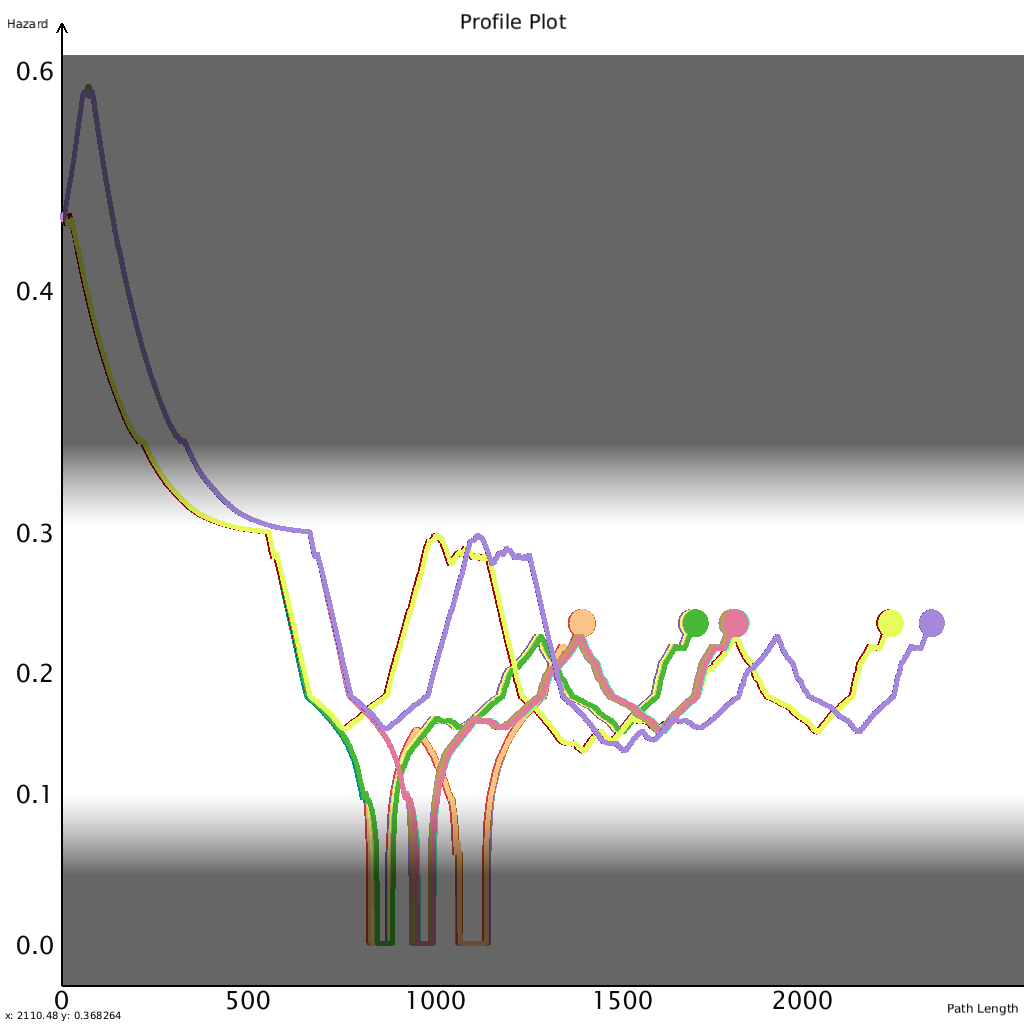
\includegraphics[width=0.45\columnwidth]{figures/fig-analysis-profile.png}}
	    \label{fig:overview:analysis:profile}
	}
	\hfill
	\subfigure[Parallel Coordinates Plot]{
	    \fbox{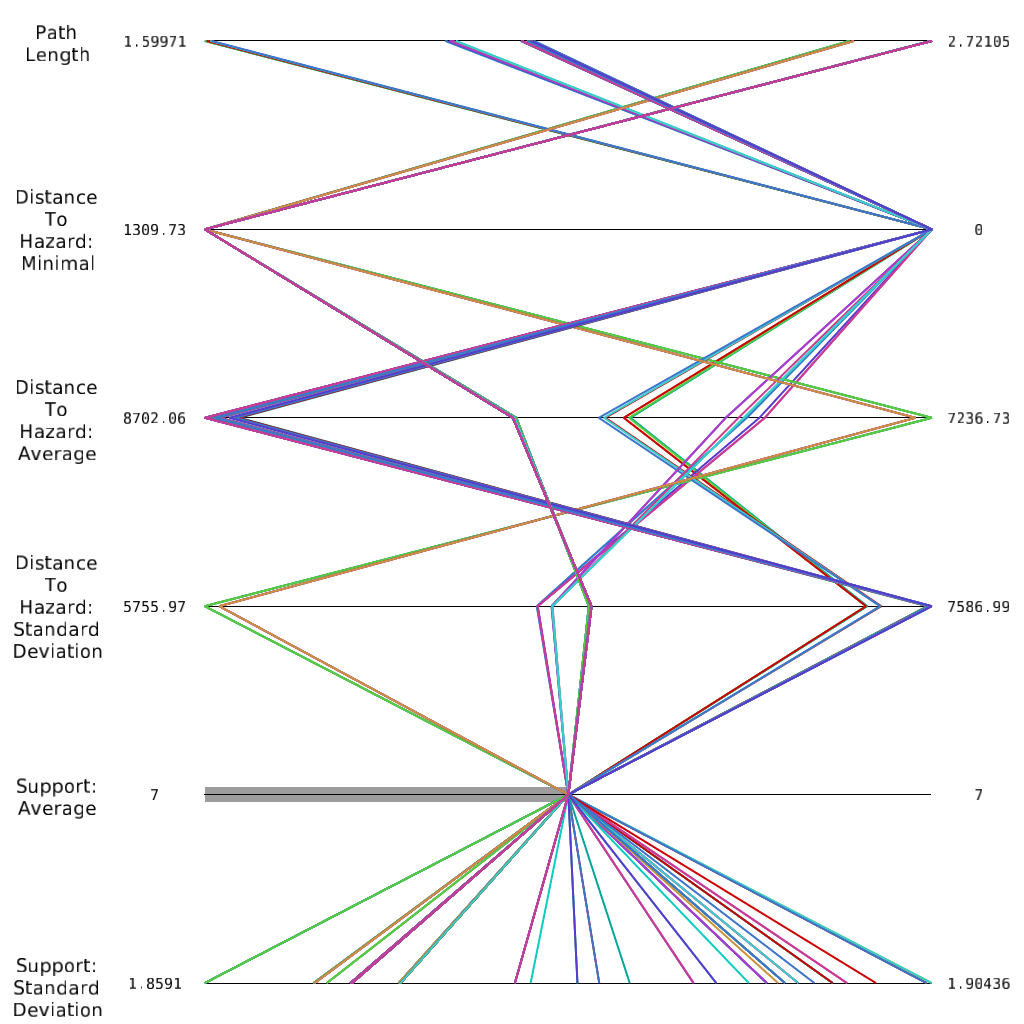
\includegraphics[width=0.45\columnwidth]{figures/fig-analysis-pcp.png}}
	    \label{fig:overview:analysis:pcp}
	}
	\caption{̄Views supporting comparative path analysis. (a) The Profile Plot presents the change of an attribute along paths; here the distance to the closest hazard. (b) Parallel Coordinates Plot showing correlations between attributes.}
\end{figure}

%%%%%%%%%%%%%%%%%%%%%%%%%%%%%%%%%%%%%%%%%%%%%%%%%%%%%%%%%%%%%%%%%%%%%%%%%%%%%%%%%%%%%%%%%%%
%%%%%%%%%%%%%%%%%%%%%%%%%%%%%%%%%%%%%%%%%%%%%%%%%%%%%%%%%%%%%%%%%%%%%%%%%%%%%%%%%%%%%%%%%%%

%\section{Implementation} \label{sec:implementation}

%In this section, we describe the details necessary to reproduce this work. %We used the OpenMP framework~\cite{660313} for most of the preprocessing and path computation and achieved a speedup that is very close to linear.

%\noindent {\bfseries Data preprocessing.} The input data is the acquired and co-registered point cloud from the autonomous robots~\cite{KohlbrecherMeyerStrykKlingaufFlexibleSlamSystem2011}. Each point in the point cloud stores its position in a global coordinate system, as well as additional information, like a color value or results from other scanners. As the global coordinate system is scanner-dependent, a transformation into a common coordinate system with standard units has to be performed. We transform the point cloud in such a way that the longest, axis-aligned side is mapped to the range $[-1,1]$. The conversion factor is stored to be later able to convert measurements back into the SI system. Based on this data the voxel binning and filtering is performed. A user-defined voxel size in SI units is prescribed and the points of the point cloud are assigned to their closest voxel center. The number of points per voxel is the occupancy, as described in Section~\ref{sec:overview:preprocessing}. The filtering step removes all voxels with an occupancy below a predefined threshold; in our case 2. This generates a second point cloud containing only the valid voxel centers. In a subsequent processing step, all attribute fields are computed for the voxel point cloud, for example normals, size restrictions, or support. These operations are performed in parallel for each voxel and do not require any intercommunication, thus providing a near-optimal parallelization. For the Tohoku dataset with 35 million points, the full pre-computation takes between two and three minutes on a four-core machine with 3\,GHz. 
%
%\noindent {\bfseries Path computation.} As described in Section~\ref{sec:overview:pathcomputation} we use the A* algorithm with the metric $m$ to generate an ensemble of paths. The parameters of the metric span a six-dimensional parameter space. We sample this space on a regular grid and compute a path for each parameter configuration. High parallelism is possible since all paths are computed independently of one another. The fields are calculated for each path and are stored alongside an ordered list of voxels, whereby for each voxel the sub-metric decision criteria are stored as well. We sampled the parameter space at about $10^5$ positions and the computations required about two minutes on a 3\,GHz four core machine. In our experiments we found that an increase to about $10^7$ positions did not yield a significant increase in usable paths as most paths started falling into distinct classes. Considering the trade-off between computational time and number of paths, we found about $10^5$ to be a good trade-off between computation time and sampling density for current machines. With respect to the parallelism, an increase in cores will lead to a linear decrease in computation time.
%
%\noindent {\bfseries 3D visualization.} The 3D visualizations are generated based on the preprocessed point cloud using OpenGL 4. The positions of the occupied voxel centers are stored in a vertex buffer object and rendered with a single \texttt{glDrawArrays} command. The different fields (see Figure~\ref{fig:overview:precomputation}) are stored in VBOs and attached as vertex attributes. The vertex shader performs packing of these values to increase the performance when the vertices are pushed through the pipeline. Although this operation reduces the dynamic range for the fields to 8 bits, the visual difference is minimal. As the size of the binning is known, a geometry shader constructs the vertices for an axis-aligned bounding box around each center, thus rendering the front faces of the boxes without the need for additional storage on the GPU. With all optimizations we achieve frame rates of at least $20$\,fps for our datasets on a GeForce GTX 580 graphics card.

%%%%%%%%%%%%%%%%%%%%%%%%%%%%%%%%%%%%%%%%%%%%%%%%%%%%%%%%%%%%%%%%%%%%%%%%%%%%%%%%%%%%%%%%%%%
%%%%%%%%%%%%%%%%%%%%%%%%%%%%%%%%%%%%%%%%%%%%%%%%%%%%%%%%%%%%%%%%%%%%%%%%%%%%%%%%%%%%%%%%%%%

\section{Results} \label{sec:results}
\begin{figure*}
\centering
   \subfigure[A construction site with an ensemble of paths starting from a construction worker standing on the edge of the pit.] {
       \fbox{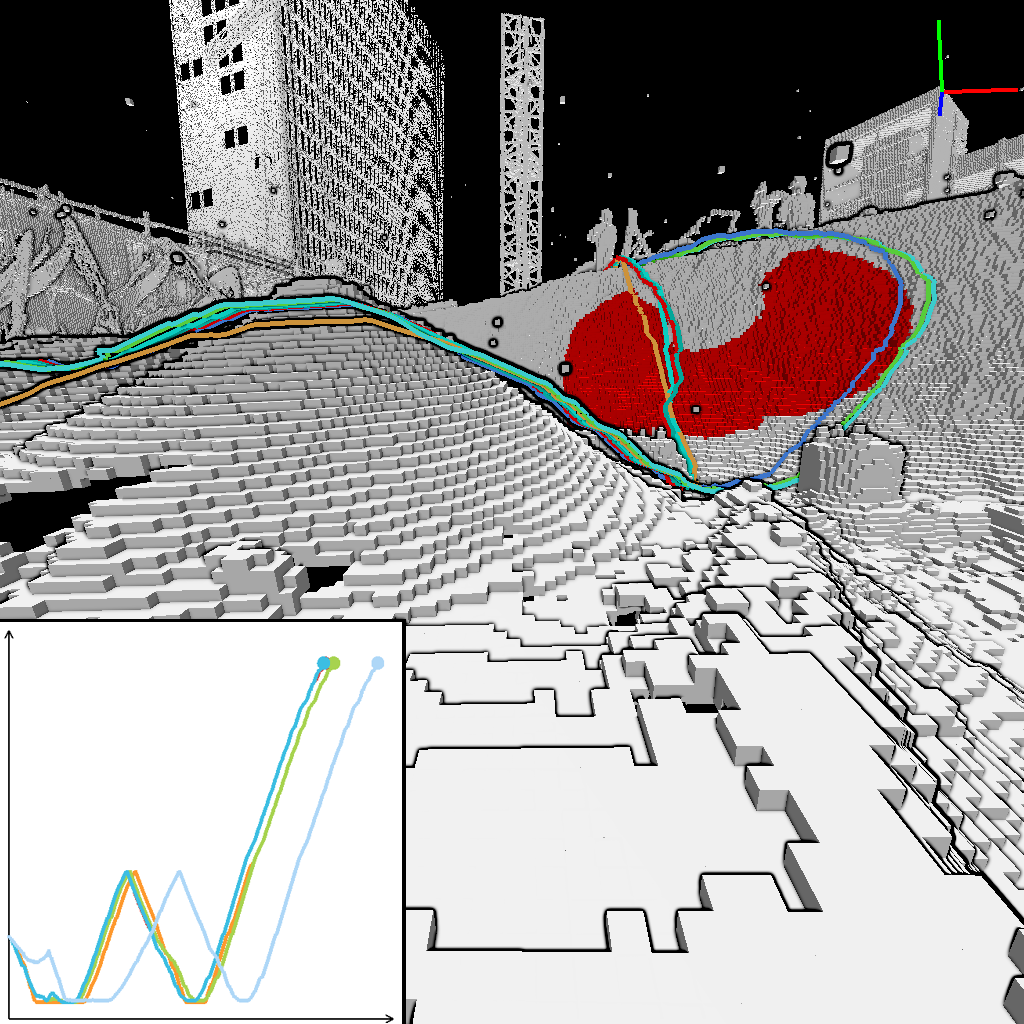
\includegraphics[width=0.3\textwidth]{figures/tower-case-path.png}}
    \label{fig:overview:case:tower}
    }
    \hfill{}
    \subfigure[An ensemble of paths calculated in the Bremen rescue arena, which is used to test the autonomy of search \& rescue robots.] {
        \fbox{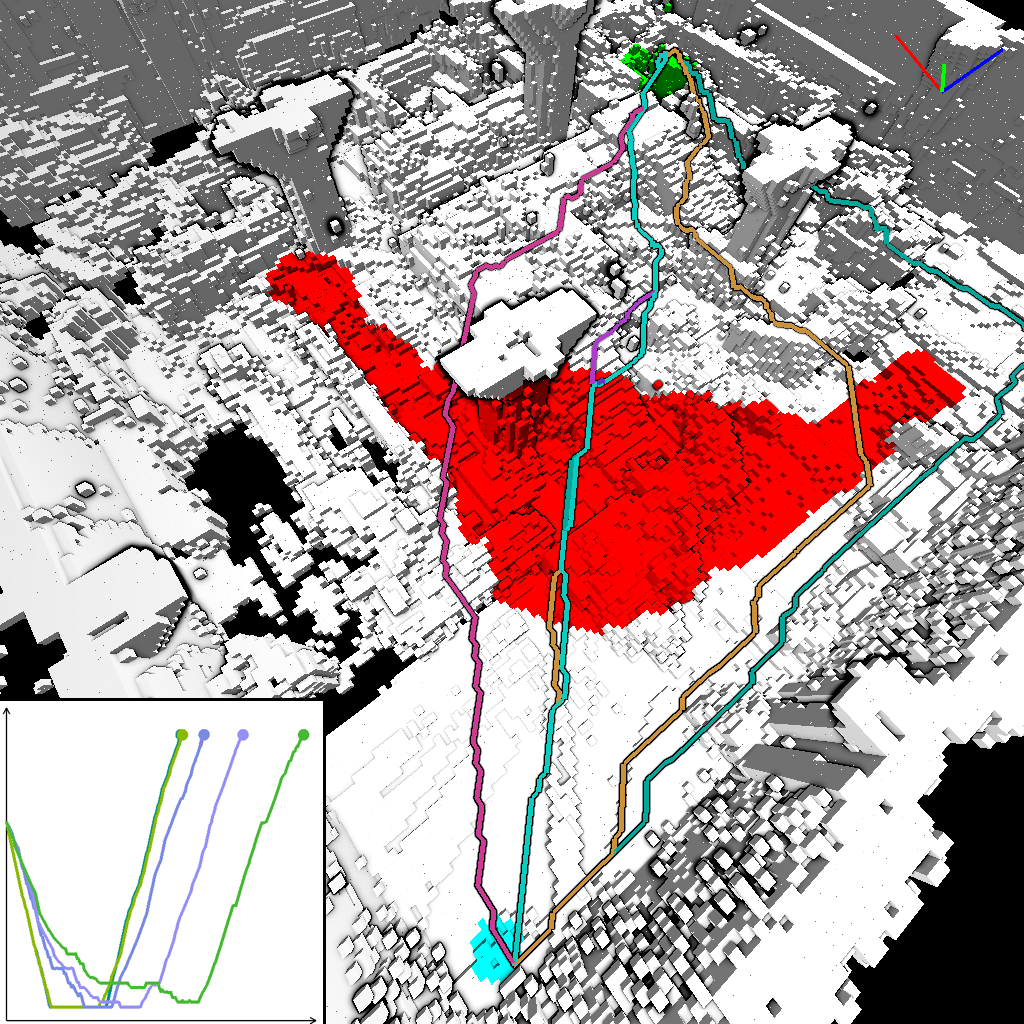
\includegraphics[width=0.3\textwidth]{figures/rescue-case-path.png}}
        \label{fig:overview:case:arena}
   }
   \hfill{}
    \subfigure[An intermediate result of the path computation in the Tohoku case showing three classes of paths through the structure.]{
        \fbox{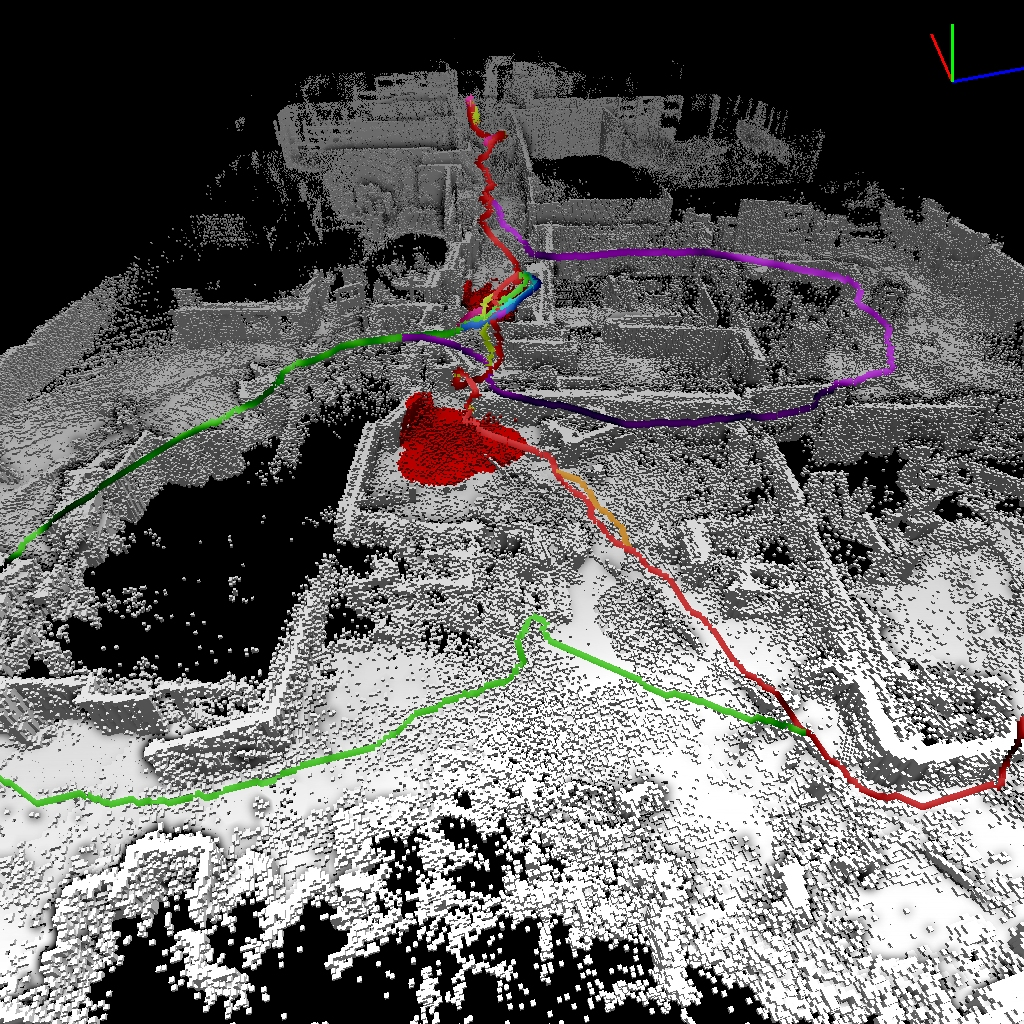
\includegraphics[width=0.3\textwidth]{figures/fig-analysis-rendering.jpg}}
        \label{fig:overview:analysis:paths}
    }
    \caption{Our system's rendering component during use in the application case (a) and the two test cases (b) and (c). The filtered paths are shown into the 3D rendering to provide an increased spatial awareness. Different weights for hazards lead to distinct optimal paths to the POI.}
\end{figure*}

Since autonomous robots are not yet used in emergency situations, it is not possible to apply our system to a real-world disaster. Instead, to illustrate the flexibility of our system, we apply the application to one application case and two test cases.

\subsection{Test Cases} \label{sec:results:testcases}
\noindent {\bfseries Construction site.} Figure~\ref{fig:overview:case:tower} shows a point cloud acquired at a construction site with a LiDAR scanner inside an excavation pit. We resampled the original dataset from $50$ million points to $3.5$ million voxels with a size of 5\,cm. The pre-computation steps took 3.5 minutes on a 3\,GHz four-core CPU.

\noindent {\bfseries Rescue arena.} Figure~\ref{fig:overview:case:arena} shows paths through the Bremen rescue arena, which is used to challenge autonomous vehicles. The original point cloud consists of $28$ million points, binned to $5.3$ million points with 4\,cm resolution. This computation took 2 minutes on the same machine as above.

\subsection{Tohoku Application Case} \label{sec:results:applicationcase}
The application case is a collapsed building at Tohoku university in the aftermath of the 2011 earthquake. The resulting dataset has been acquired with latest state-of-the-art equipment~\cite{journals/jfr/NagataniKOOYTNYKFK13} and consists of $26$ million sampling points, resampled to $4$ million voxels with a size of 3\,cm. It proved to be a valid and useful simulated real-world application case to test our proposed system due to partial collapses causing uneven ground and obstacles. Figure~\ref{fig:teaser:1} shows a closeup rendering showing that the level of detail is sufficient to support spatial awareness. Figure~\ref{fig:teaser:2} shows an overview of the scanned area with the POI in green at the top. No hazards were detected by the robots during the acquisition as this was not part of their mission profile. The task for this application case was as follows: the \IC\ needed to find the shortest path between the entry point and the POI. While traversing the path, a rescuer would detect two hazards (highlighted in red) and the system must be able to react to this changing situation. In Figure~\ref{fig:overview:analysis:paths}, a subset of computed paths is shown after the discovery of the second hazard. There is one class of paths (purple) that evades the first hazard and another class (green) that evades the second hazard. The parallel coordinates plot (Figure~\ref{fig:overview:analysis:pcp}) makes it possible to detect paths belonging to both classes with a maximum in the \emph{Minimal Hazard Distance}, while having a long \emph{Path Length}.

%%%%%%%%%%%%%%%%%%%%%%%%%%%%%%%%%%%%%%%%%%%%%%%%%%%%%%%%%%%%%%%%%%%%%%%%%%%%%%%%%%%%%%%%%%%
%%%%%%%%%%%%%%%%%%%%%%%%%%%%%%%%%%%%%%%%%%%%%%%%%%%%%%%%%%%%%%%%%%%%%%%%%%%%%%%%%%%%%%%%%%%

\section{Evaluation} \label{sec:evaluation}
We performed an evaluation of our system with nine external experts. Of these experts, five (A--E) are emergency responders, three (F--H) are researchers, and one (J) is a consultant for a national technical relief agency. As the goal of the study was to include many international experts, and being aware of their time constraints, we created an interactive webpage featuring videos and images of our system rather than requiring the training for a hands-on use. The experts had to inspect images and/or videos and then reply to questions and give feedback without a time limit. 7 of 9 experts finished the evaluation and provided answers to all questions. We have considered partial responses where an answer was provided.

The feedback is grouped into four categories; first, questions letting the experts assess their own knowledge about the component. With these questions, we can estimate whether the experts have prior knowledge and how intuitive the component is. The replies to these questions are on a 5-point Likert scale. The second category are factual checks that have a correct answer. These are used to test if the experts' self-assessment is accurate. The third type of questions are open-ended and allow us insight into the experts' thinking process. Usually, these questions do not have a best answer, but require a trade-off and domain knowledge. The fourth category asks for general comments about a component. The full evaluation and replies are available in the supplemental material. Here, we will discuss important positive and negative answers. 

\noindent \textbf{3D Representation} This component evaluates the general usefulness of the 3D rendering. A video as well as images similar to Figures~\ref{fig:teaser:1},~\ref{fig:teaser:2}, and~\ref{fig:overview:analysis:paths} were provided. We asked to rate the degree of immersion (average: 2.94), the level of knowledge the experts had acquired (average: 2.5), and if the 3D rendering was useful in general (average: 4.14). To test the level of immersion and knowledge of the scene, we asked the experts to describe the room shown in the images, which all performed successfully, leading us to believe that the experts underestimated the knowledge they gained from the 3D rendering. An outlier in the responses was F, who reported 1 for the knowledge and 5 for the usefulness, but described the room correctly. We assume the answers are related to his comment, asking us to ``improve [our] registration algorithm''. \\
%
\noindent \textbf{Path Representation} This component tests the usefulness of embedding the paths into the rendering. It consists of three images depicting the same situation as Figure~\ref{fig:teaser:2}. The first scenario with no hazardous areas, the second with the upper hazard only, and the third with both hazards. We asked the experts which of the paths they would choose. All but two (A and F) chose the paths that evaded the hazards. A second question was asked to compare the lengths of the shortest and the longest path. The correct answer was 1.54$\times$, while the experts stated an average of 2.56$\times$. This means that, while the experts are capable of estimating the length within a reasonable margin of error, they overestimate path distances, making it necessary to provide accurate information in the PP and PCP. \\
%
\noindent \textbf{Evacuation Path Walkthrough} In this component, we evaluated the combined effects of the first two components. We generated two camera paths from the longest path in component 2; one path moving from the \emph{Start} to the \emph{POI} and a second moving opposite. We asked for the usefulness (average: 3.125) and the self-assessed knowledge (average: 2.75) for both paths. \\
%
\noindent \textbf{Profile Plot} We provided a plot containing the orange, green, and yellow paths from Figure~\ref{fig:overview:analysis:profile}. We asked for the assessment of understanding (average: 3.5) and the usefulness (average: 3.71). Asking for the shortest path, and the number of times it crosses the hazard, all experts gave correct answers. \\
%
\noindent \textbf{Parallel Coordinates Plot} The self-assessed understanding is significantly lower compared to the PP (average: 1.66) which can be attributed to the experts' unfamiliarity with PCPs. Correct answers, however, show that the PCP can still be a valid and useful component in our system. Despite their unfamiliarity, all five experts providing feedback found the shortest and the safest path, identifying the path with the lowest path length and the highest minimal distance. In the open questions, the experts seemed to favor safe, long paths over shorter, more dangerous paths while not paying much attention (except J) to the available support. This confirmed our design fixing the attribute ordering in the PCP. The experts rated the usefulness of the PCP with an average of 2.14. \\
%
\noindent \textbf{Scatterplot Matrix} The SPLOM received a very low level of self-assessed knowledge (average: 1.16) and usefulness (average: 1.28). Though this might be, just as the PCP, due to the fact that few, if any, have worked with SPLOMs before. A comment from E summarizes this component's result: ``[this] is more information than I would want to interpret during a SAR mission''. Given the experts' replies, the SPLOM component is an optional component of our system. \\
%
\noindent \textbf{Miscellaneous} For the last part, we asked if it is ``helpful to display the paths and [if it] provides additional information'', to which most experts (C, D, E, F, and J) agreed. D noted that the GUI should be more ``user-friendly and understandable'' and J said that ``not detected hazards like structural integrity get visible by the density of scan points''. To the question if they ``[would] like to use [the] system in addition, or as a replacement, to [their] current tools'', B, C, E, F, and J were positive to using our system in addition to their current tools rather than as a replacement. C would like to use it after a ``period of experimentation'', while J sees the system as ``an addition which is warmly welcome''. The only negative comment was from D, who regards the system as too complicated. J suggested a collaboration, saying that the system needs to be more intuitive to allow rescuers, who do not work with SAR operations regularly, to use its full potential.

We received valuable feedback from the experts and we can draw the conclusion that most experts liked the system and would like to use it as a decision-support tool alongside their current applications. With the exception of the SPLOM, the majority of experts were able to retrieve information from our system and use it for their decision-making.

%%%%%%%%%%%%%%%%%%%%%%%%%%%%%%%%%%%%%%%%%%%%%%%%%%%%%%%%%%%%%%%%%%%%%%%%%%%%%%%%%%%%%%%%%%%
%%%%%%%%%%%%%%%%%%%%%%%%%%%%%%%%%%%%%%%%%%%%%%%%%%%%%%%%%%%%%%%%%%%%%%%%%%%%%%%%%%%%%%%%%%%

\section{Conclusions} \label{sec:conclusion}
We presented a linked, multiple-view visualization system that optimizes the workflow of an incident commander when dealing with search \& rescue missions in cases where the initial reconnaissance of a collapsed structure is performed using unmanned vehicles. Based on this data, our system computes and analyzes an ensemble of rescue paths that are explored by the \IC , who can then select a path that is an optimal trade-off according to his experience and knowledge. To investigate the system's usefulness, we have conducted a study with experts. The resulting positive feedback makes us confident that the system has the potential to improve future search \& rescue planning missions. In addition, we presented a stereoscopic movie of the application case and the rescue arena data sets to an audience of approximately 100 researchers at an IEEE-sponsored conference on rescue robotics (see Figure~\ref{fig:cloud:dome}). We received positive informal feedback from these research experts on the rendering over the course of later discussions.

%We like to thank the IRIDeS, the CREATE, and the IRS institutes for their cooperation in retrieving and providing the scans from Tohoku university.

%For future work, we like to perform a thorough in-use evaluation accompanying a real-world rescue scenario. This will provide us with valuable direct feedback to improve usability of the system. Furthermore, we plan to investigate the applicability of adaptive and stochastic sampling, like Monte-Carlo methods, on the high-dimensional parameter space for path computation.

%%%%%%%%%%%%%%%%%%%%%%%%%%%%%%%%%%%%%%%%%%%%%%%%%%%%%%%%%%%%%%%%%%%%%%%%%%%%%%%%%%%%%%%%%%%
%%%%%%%%%%%%%%%%%%%%%%%%%%%%%%%%%%%%%%%%%%%%%%%%%%%%%%%%%%%%%%%%%%%%%%%%%%%%%%%%%%%%%%%%%%%

We like to thank the IRIDeS, the CREATE, and the IRS institutes for their cooperation in retrieving and providing the scans from Tohoku university. This work was partly supported by grants from the Excellence Center at Link\"oping and Lund in Information Technology (ELLIIT) and the Swedish e-Science Research Centre (SeRC), as well as VR grant 2011-4113.
%We would like to thank the external experts for taking their time to take part in the evaluation.
The presented system has been realized using the Voreen framework (www.voreen.org).
%}

%\bibliographystyle{abbrv}
%%use following if all content of bibtex file should be shown
%\nocite{*}
%\bibliography{bibliography}

\bibliographystyle{IEEEtran}
\bibliography{bibliography}

\end{document}